\documentclass[11pt]{article}

\usepackage{comment} % enables the use of multi-line comments (\ifx \fi) 
\usepackage[a4paper,margin=1cm]{geometry}
\usepackage[utf8]{inputenc}
\usepackage[ngerman]{isodate}
\usepackage{gensymb}
\usepackage{graphicx}
\usepackage{booktabs}% http://ctan.org/pkg/booktabs
\usepackage{tabularx}
\usepackage{ltablex} % Longtables with tabularx
\usepackage[x11names]{xcolor}
\usepackage{amsmath}
\usepackage{amssymb}
\usepackage{amsthm}
\usepackage{array}
\usepackage{wrapfig}
\usepackage{subcaption}
\usepackage{pdflscape}
\usepackage{geometry}
\usepackage{multicol}
\usepackage{bm}
\usepackage{enumitem}
\usepackage{mdframed}
\usepackage{scalerel}
\usepackage{stackengine}
\usepackage{mathtools}
\usepackage{pdfpages}
\usepackage[normalem]{ulem}

% Code highlighting
\usepackage{minted}
\usepackage{pythonhighlight}
\surroundwithmdframed{minted}

% Be able to caption equations and float them in place
\usepackage{float}

\usepackage{csquotes}
\usepackage{hyperref}

\newmdtheoremenv{theorem}{Theorem}

\theoremstyle{definition}
\newmdtheoremenv{definition}{Definition}[section]

\geometry{a4paper, margin=2.4cm}

\newcommand\equalhat{\mathrel{\stackon[1.5pt]{=}{\stretchto{\scalerel*[\widthof{=}]{\wedge}{\rule{1ex}{3ex}}}{0.5ex}}}}
\newcommand\defeq{\mathrel{\overset{\makebox[0pt]{\mbox{\normalfont\tiny def}}}{=}}}
\newcolumntype{C}{>{\centering\arraybackslash}X}

\DeclarePairedDelimiter\abs{\lvert}{\rvert}
\DeclarePairedDelimiter\norm{\lVert}{\rVert}

\newcommand*\samplemean[1]{\overline{#1}}
\newcommand*\ev[1]{\mathrel{\text{E}\left[#1\right]}}
\newcommand*\R{\mathbb{R}}
\newcommand*\Z{\mathbb{Z}}
\newcommand*\N[1]{\mathcal{N}\left(#1\right)}
\newcommand*\F[1]{\mathcal{F}_{#1}}
\newcommand*\Likelihood{\mathcal{L}}
\newcommand*\diff{\mathop{}\!\mathrm{d}}
\newcommand*\Diff[1]{\mathop{}\!\mathrm{d^#1}}
\newcommand*\Exp[1]{\mathop{\text{Exp}}\left(#1\right)}
\newcommand*\Cov[1]{\mathop{\text{Cov}}\left(#1\right)}
\newcommand*\Cor[1]{\mathop{\text{Cor}}\left(#1\right)}
\newcommand*\Var[1]{\mathop{\text{Var}}\left(#1\right)}

\setcounter{tocdepth}{3}
\setcounter{secnumdepth}{3}

\graphicspath{{./img/}}

\begin{document}
	
\title{Machine Learning in Computer Vision FS20}
\author{Pascal Baumann\\pascal.baumann@stud.hslu.ch}
\maketitle



For errors or improvement raise an issue or make a pull request on the \href{https://github.com/KilnOfTheSecondFlame/mse_summaries}{github repository}.

\tableofcontents
\newpage


\section{Image Handling in Python}

\begin{minted}[tabsize=2]{python}
plt.imshow(np.hstack((im_float, im_float)), cmap="gray", vmin=0, vmax=1);
\end{minted}

\begin{center}
	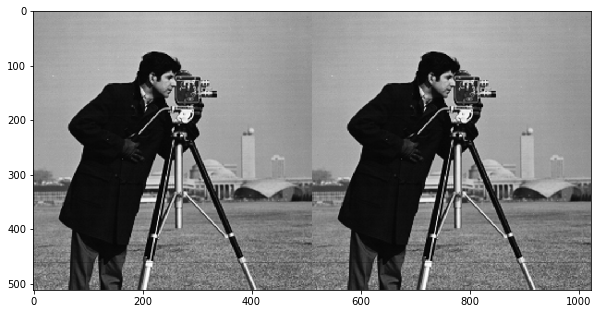
\includegraphics[width=0.7\linewidth]{img/hstack_image}
\end{center}

\subsection{Fading an Image}
\begin{minted}[tabsize=2]{python}
im = skimage.io.imread("data/snoopy.png")
im = im/255 # tip: use floating point values

ims = []

im_temp = np.fliplr(im)
ims.append(im_temp)
for i in range(1,5):
	im_temp = im_temp + (0.4)**i
	ims.append(im_temp)

plt.imshow(np.hstack(ims),vmin=0, vmax=1, cmap="gray")
\end{minted}

\begin{center}
	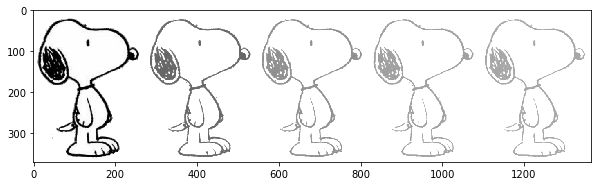
\includegraphics[width=0.7\linewidth]{img/snoopy_fade}
\end{center}

\subsubsection{IPyWidgets}
\begin{minted}[tabsize=2]{python}
@interact(thresh=widgets.FloatSlider(min=0.0, max=0.5, step=0.01, value=0.2))
def threshold(thresh):
	im_thresh = []
	for line in im:
		im_thresh.append([pixel if pixel > np.min(line) 
			+ thresh else float(0) for pixel in line])
	plt.imshow(im_thresh, cmap="gray", vmin=0, vmax=1)
	plt.show()
\end{minted}

\begin{center}
	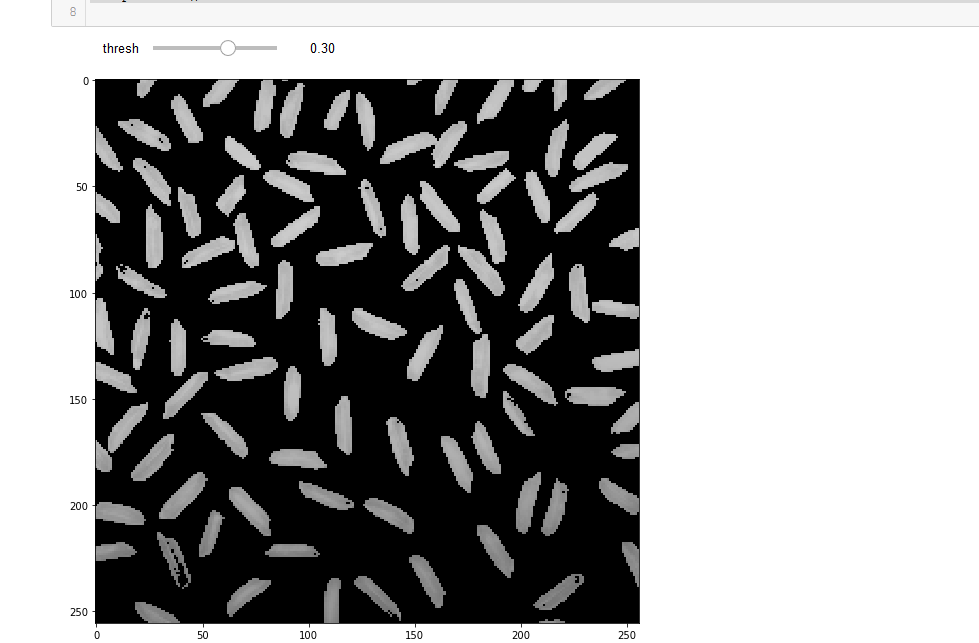
\includegraphics[width=0.6\linewidth]{img/ipywidgets_example}
\end{center}

\section{Local Filtering and Edge Detection}
\subsection{Filtering}
The naive approach of local filtering is taking just a moving average of the pixels in the neighbourhood.

\subsection{Edge Detection}
Although intuitive for humans to detect, edge detection was a hard problem in image processing. And edge is defined by a rapid change in the intensity, which can be exploited by calculating the derivative.

\begin{center}
	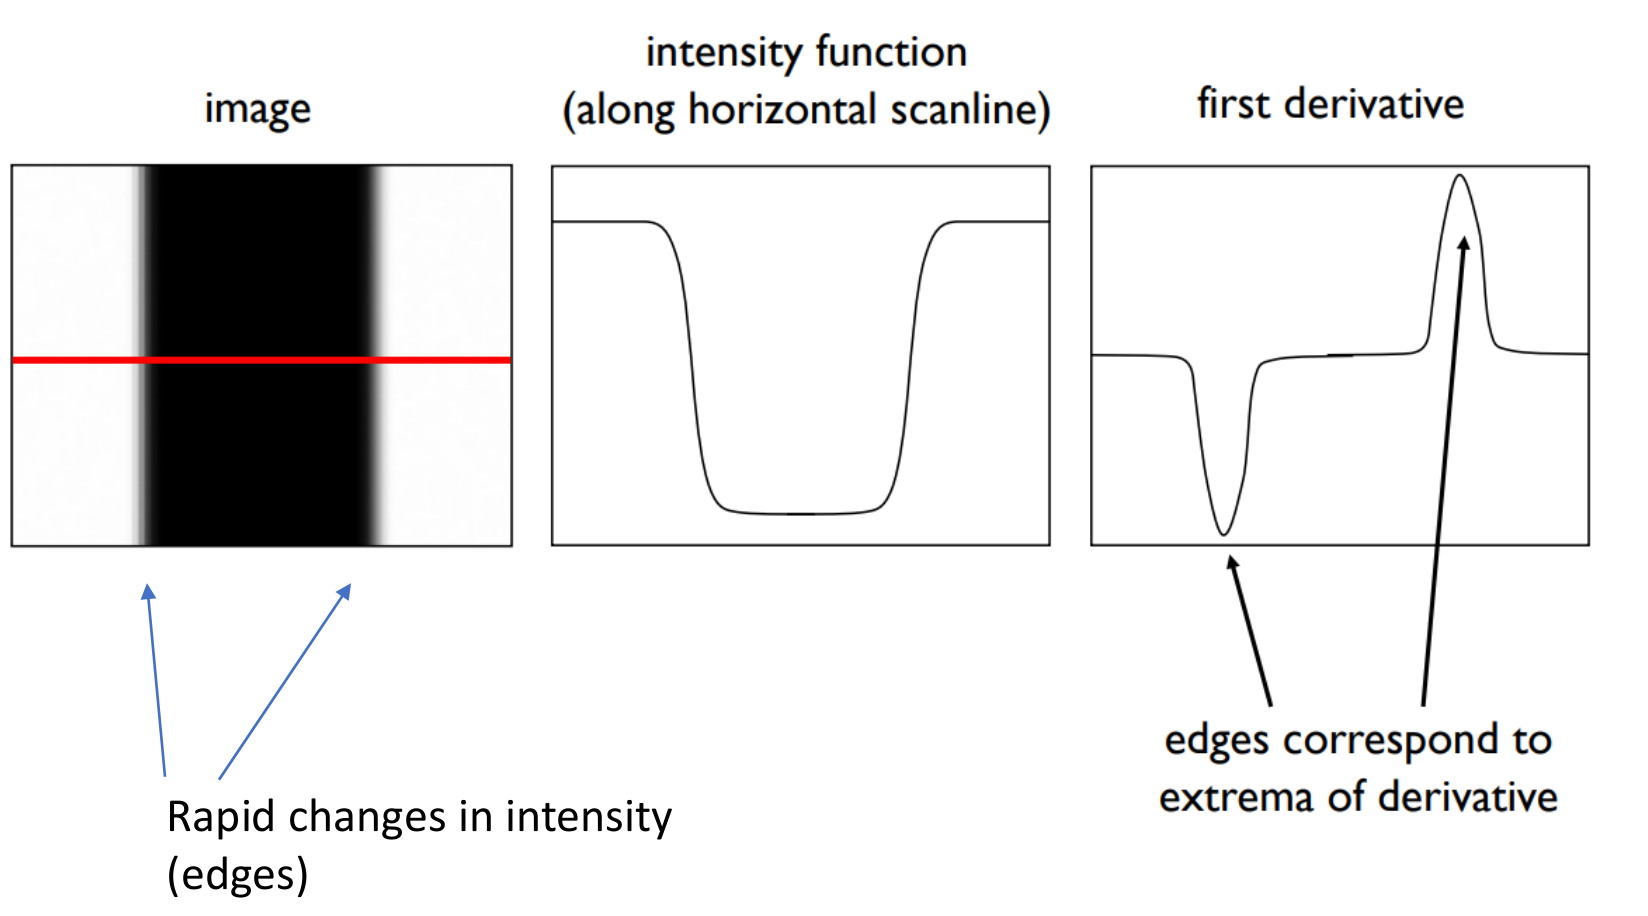
\includegraphics[width=0.6\linewidth]{img/1D_edge_derivative}
\end{center}

\noindent
In two dimensions the derivative corresponds to the gradient $\nabla f = \left[\frac{\partial f}{\partial x},\frac{\partial f}{\partial y}\right]$, which points from the edge towards the increase in intensity or the lighter side.

\begin{align}
\shortintertext{Gradient}
\nabla f &= \left[ \frac{\partial f}{\partial x}, \frac{\partial f}{\partial y} \right]
\shortintertext{Gradient Direction}
\theta &= \tan^{-1} \left( \frac{\partial f}{\partial x} / \frac{\partial f}{\partial y} \right)
\shortintertext{Gradient Magnitude (strength of the edge)}
\norm{\nabla f} &= \sqrt{\left(\frac{\partial f}{\partial x}\right)^2 + \left(\frac{\partial f}{\partial y} \right)^2 }
\end{align}

But not all important edges have strong gradients, nor are all strong gradients important edges.

\subsubsection{Computing the Gradient on an Image}
Approximate Gradient in direction of $ \frac{\partial f}{\partial x} $: Convolution with kernel \begin{tabular}{|c|c|}
	\hline
	-1 & 1\\
	\hline
\end{tabular}

\noindent
Approximate Gradient in direction of $ \frac{\partial f}{\partial y} $: Convolution with kernel \begin{tabular}{|c|}
	\hline
	-1 \\
	\hline
	1\\
	\hline
\end{tabular}

The drawback of the gradient is, that it is very sensitive to noise:
\begin{figure}[H]
	\centering
	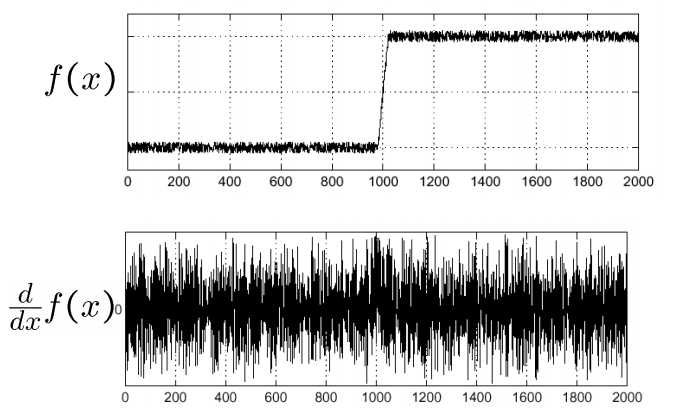
\includegraphics[width=0.7\linewidth]{noise_gradient}
	\caption{Gradient of a 1D function, where it is clear how it amplifies noise and may conceal a weak signal}
	\label{fig:noisegradient}
\end{figure}

\noindent
The solution to this is, to first smooth the function and then apply the gradient.

The larger the value of $\sigma$ the more smoothing is applied and different kind of features can be identified.
\begin{itemize}[leftmargin=*, labelindent=3.5cm, labelsep=0.5cm]
	\item[\textbf{large value of $\sigma$}] larger scale or stronger edges detected
	\item[\textbf{smaller value of $\sigma$}] finer details detected
\end{itemize}

\noindent
\begin{minipage}{0.6\textwidth}
	In practice a convolution with a derivative of Gaussian filter is calculated to compute the gradients.
	
	This is equivalent to smoothing with a Gaussian and then taking the derivative.
\end{minipage}
\begin{minipage}{0.4\textwidth}
	\begin{center}
		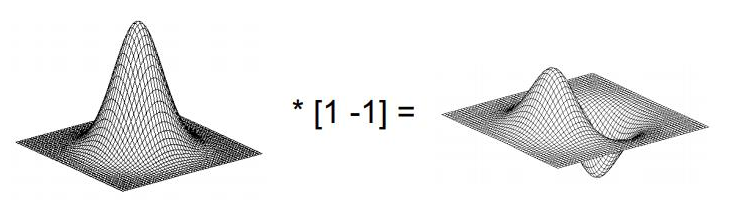
\includegraphics[width=0.6\linewidth]{img/derivative_gaussian_filter}
	\end{center}
\end{minipage}

\begin{figure}[H]
	\centering
	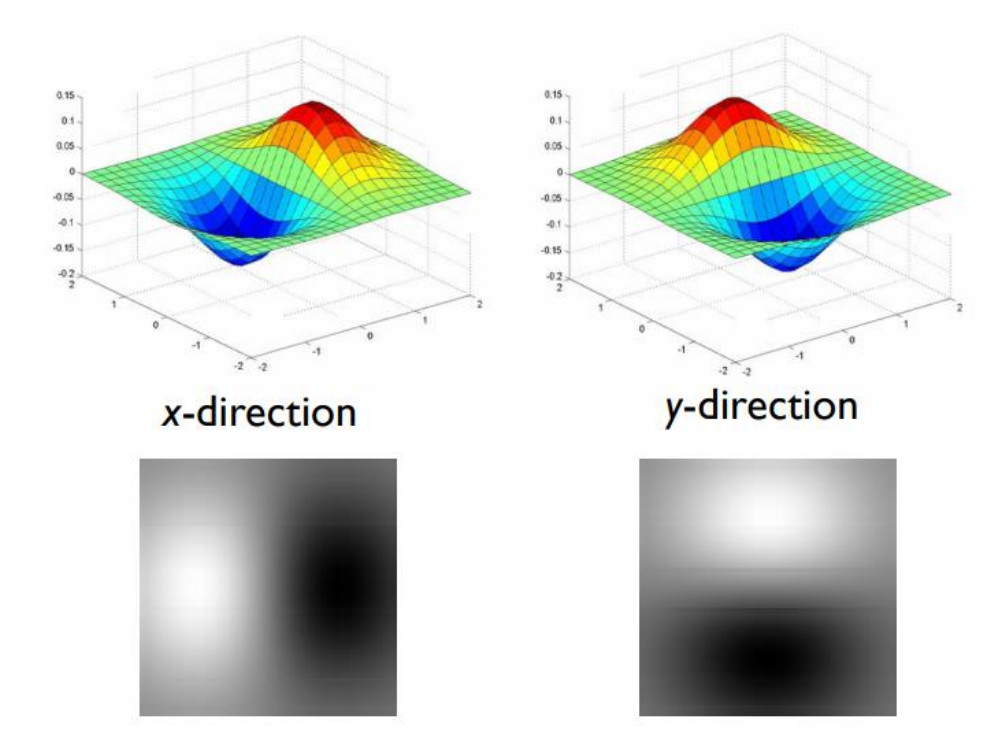
\includegraphics[width=0.6\linewidth]{img/derivative_gaussian_filter2}
	\caption{Derivative of Gaussian Filters}
	\label{fig:derivativegaussianfilter2}
\end{figure}

\begin{itemize}
	\item A Gaussian smoothing filter removes high-frequency components
	\item Values of a Gaussian smoothing filter sum to one
	\item Derivative filters contain some negative value and values sum to zero
	\item Derivative filters yield large responses at points with high contrast
\end{itemize}

\subsection{Canny Edge Detection}
Same base approach but enhanced with edge thinning and hysteresis thresholding.
\begin{enumerate}
	\item Approximate gradients along axes by derivative of Gaussian filters
	\item Compute gradient magnitude
	\item Make edge one pixel wide, thinning through \textbf{non-maxima suppression} along perpendicular direction to wthe edge
	\item Only keep strong edges through hysteresis thresholding 
\end{enumerate}

\subsection{Hysteresis Thresholding}
This stage decides which are all edges are really edges and which are not. For this, we need two threshold values, minVal and maxVal. Any edges with intensity gradient more than maxVal are sure to be edges and those below minVal are sure to be non-edges, so discarded. Those who lie between these two thresholds are classified edges or non-edges based on their connectivity. If they are connected to "sure-edge" pixels, they are considered to be part of edges. Otherwise, they are also discarded.
	
\begin{figure}[H]
	\centering
	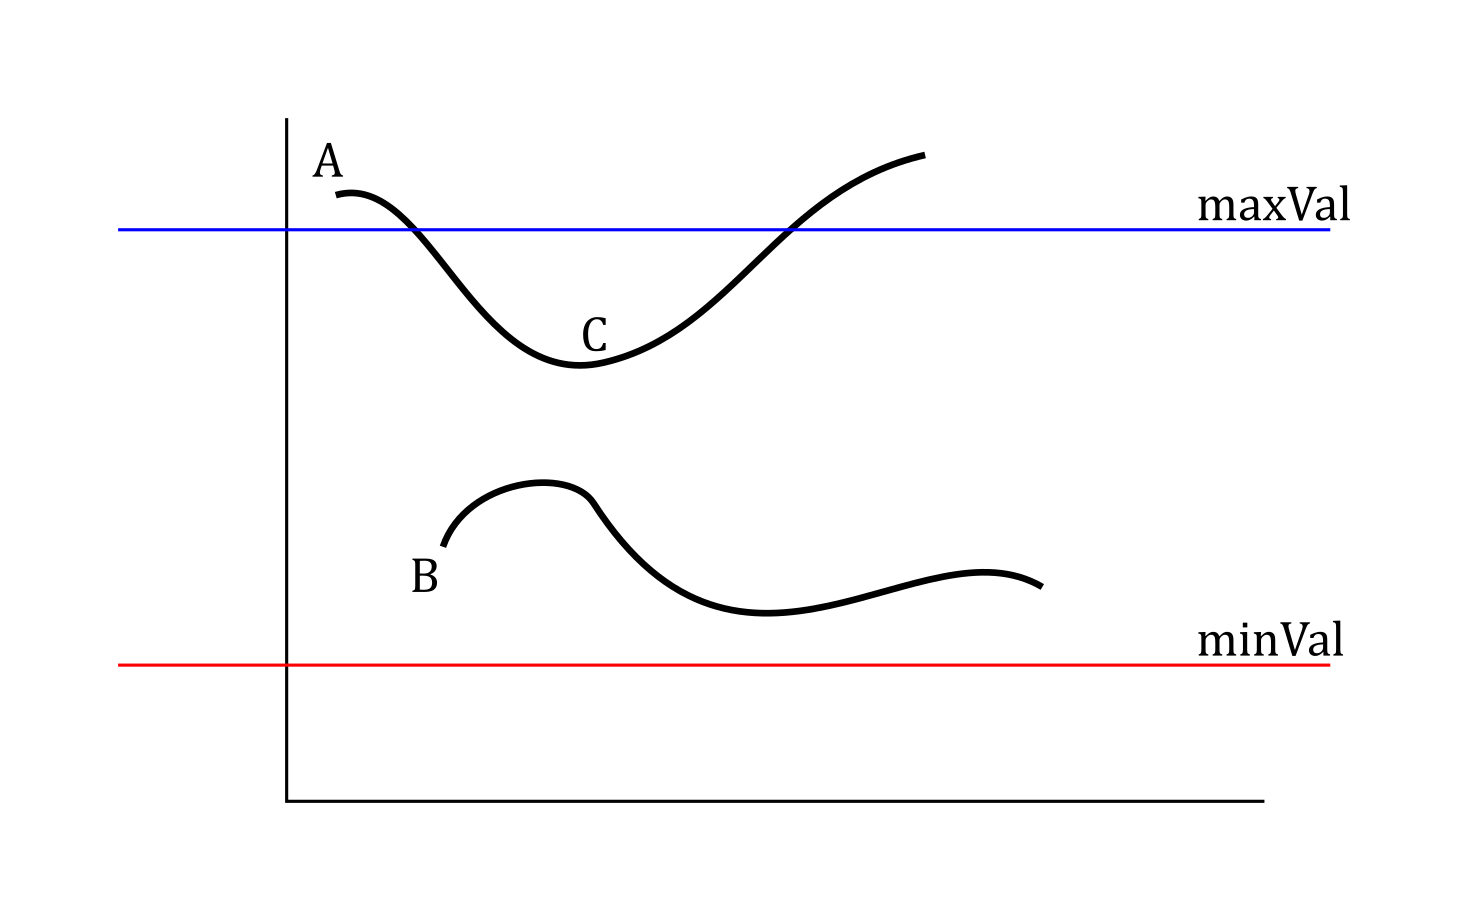
\includegraphics[keepaspectratio,width=0.6\linewidth]{hysteresis_thresholding}
	\caption{Hysteresis thresholding with A) sure edge, B) non-edge and C) a non-edge connected to a sure edge}
\end{figure}

\section{Model Fitting and Line and Circle Detection}
Edge detection is usually not enough as there are usually more than one line in an image and many edges that do not belong to a line. There might be noise in the edges belonging to a line which brings them out of alignment. Lines might also not be complete.

\subsection{Model Fitting}
Model fitting is an algorithm finds or fits a high-level explanation or model that explain the observation well. In this case the edges are the observations and the model are one or more line.

\subsection{Voting Algorithms}
Voting algorithms are a general technique for decision methods.

\begin{enumerate}
	\item Every feature casts votes for all models that are compatible with it
	\item Choose models that accumulate a lot of votes
\end{enumerate}

Clutter and noise will cast a lot of votes, but are inconsistent. Instead, features belonging to a model will concentrate a lot of votes for that model.

\subsection{Hough Transform}
\begin{enumerate}
	\item Every \textbf{edge point} casts votes for \textbf{all lines that are compatible} with it
	\item Choose \textbf{lines} that accumulated a lot of votes
\end{enumerate}

\begin{figure}[H]
	\centering
	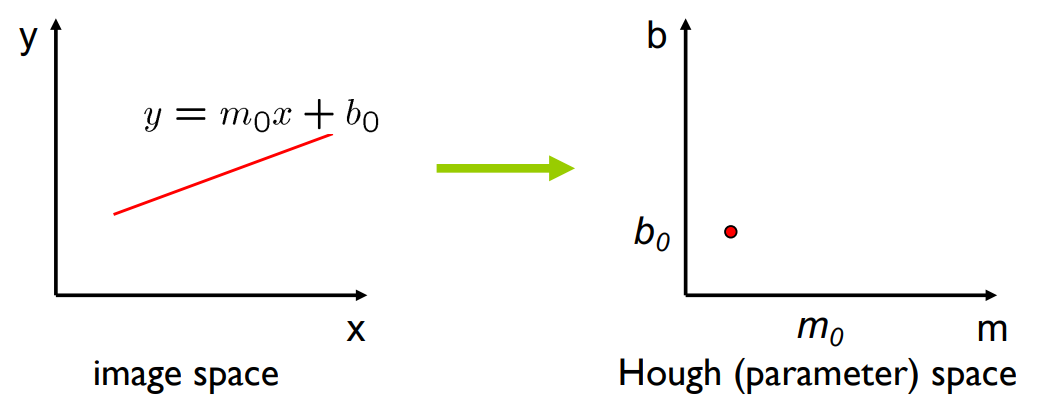
\includegraphics[width=0.8\linewidth,keepaspectratio]{img/line_representation_hough}
	\caption{Line representation in Hough space}
\end{figure}

\begin{figure}[H]
	\centering
	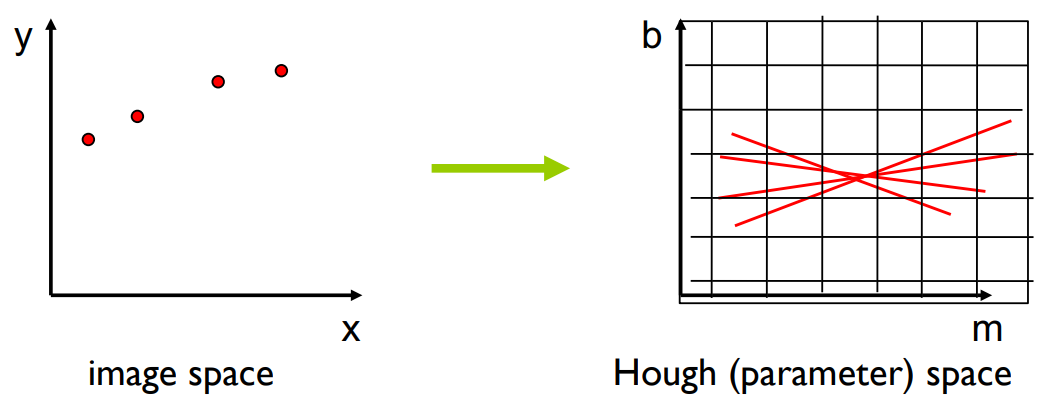
\includegraphics[width=0.8\linewidth]{img/points_representation_hough}
	\caption{Points on a line in normal space almost intersect in Hough space}
	\label{fig:pointsrepresentationhough}
\end{figure}

\noindent
The problem with this approach is that
\begin{enumerate}[label=\alph*.]
	\item the parameter space $(m,b)$ is \textbf{not bounded}
	\item \textbf{vertical lines} can not be represented
\end{enumerate}

\subsection{Representation of Lines in Polar Coordinates}

\begin{figure}[H]
	\centering
	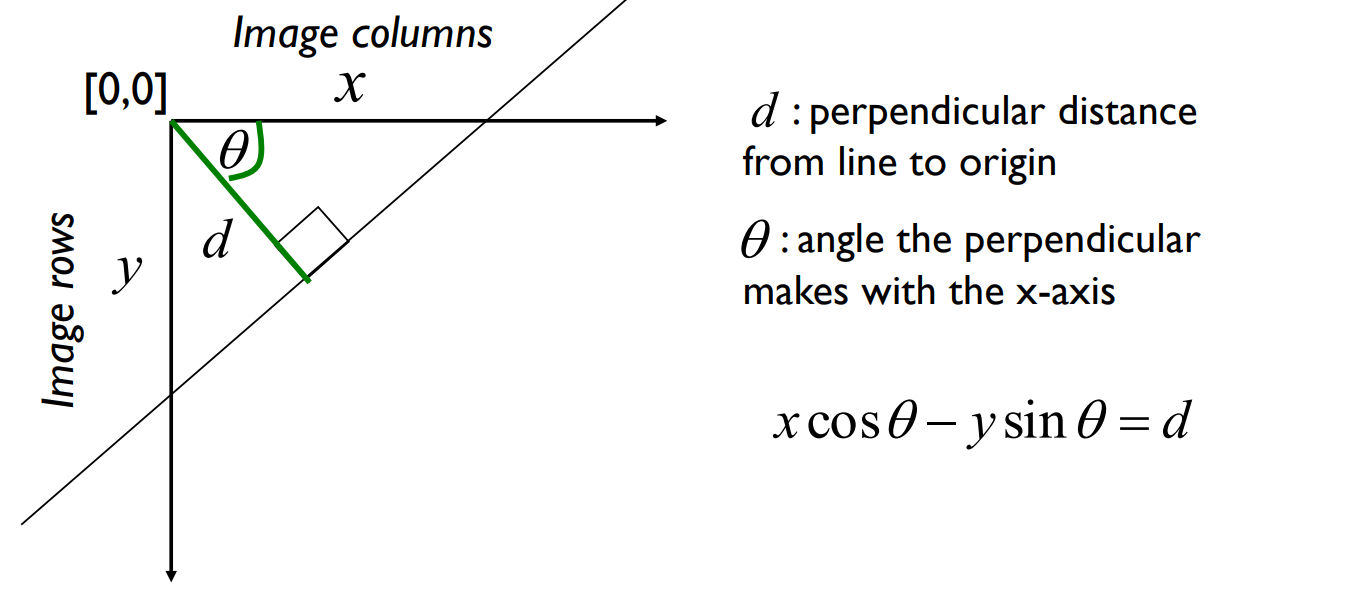
\includegraphics[width=0.8\linewidth]{img/line_representation_polar}
	\caption{Line representation with polar parameters}
	\label{fig:linerepresentationpolar}
\end{figure}

This approach solves both the problem of unboundedness and representation. The parameter $\theta$ is bounded by $[0,2\pi]$ and $d$ by $[0,\text{imagewidth}]$.

For every point in normal space there will be a Sinusoid the polar Hough space.

\subsection{Hough Transformation Algorithm}
The algorithm transforms each edge point in the image to the Hough space, where an Accumulator array gets filled with votes. The bin size of the accumulator is an important hyperparameter, if the size is too small, there will be many weak peak due to noise, if too large accuracy of locating a line drops and many votes from clutter might end up in the same bin. A solution is to keep the bin size small but also count votes from neighbours.

% TODO Hough circles

\subsubsection{Voting Algorithm for Finding Lines}
\begin{enumerate}
	\item Every edge point casts votes for all circles that are compatible with it
	\item We choose circles that accumulated a lot of votes
\end{enumerate}

\begin{theorem}
	Parametrisation of a circle
	\begin{equation*}
		(x_i - a)^2 + (y_i - b)^2 = r^2
	\end{equation*}
	With centre $(a,b)$ and radius $r$
\end{theorem}

\begin{center}
	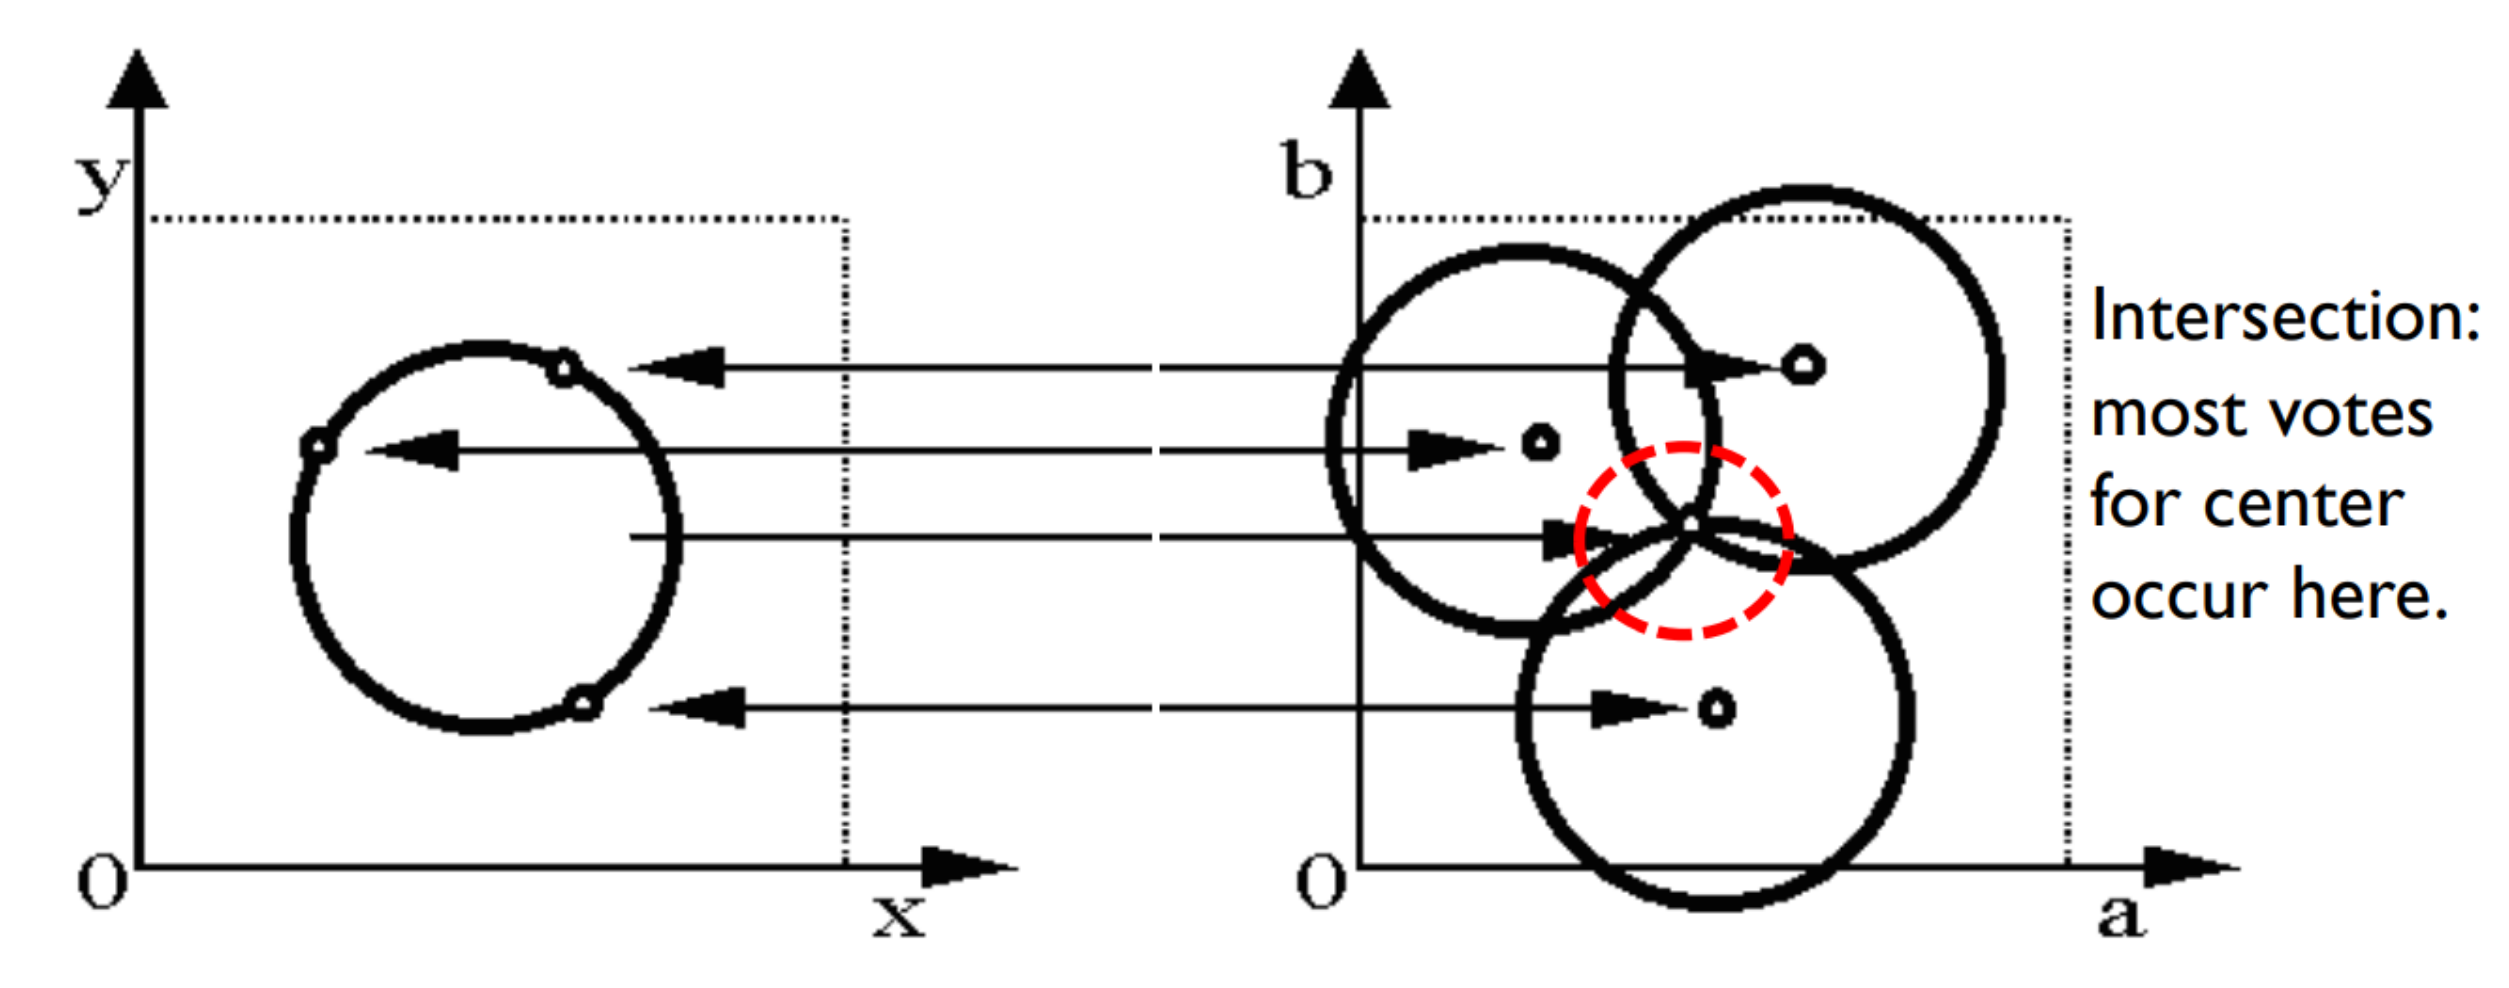
\includegraphics[width=0.7\linewidth]{img/hough_circle_accumulator}
\end{center}

\subsection{Hough Space for Circles With Unknown Radius}

\begin{center}
	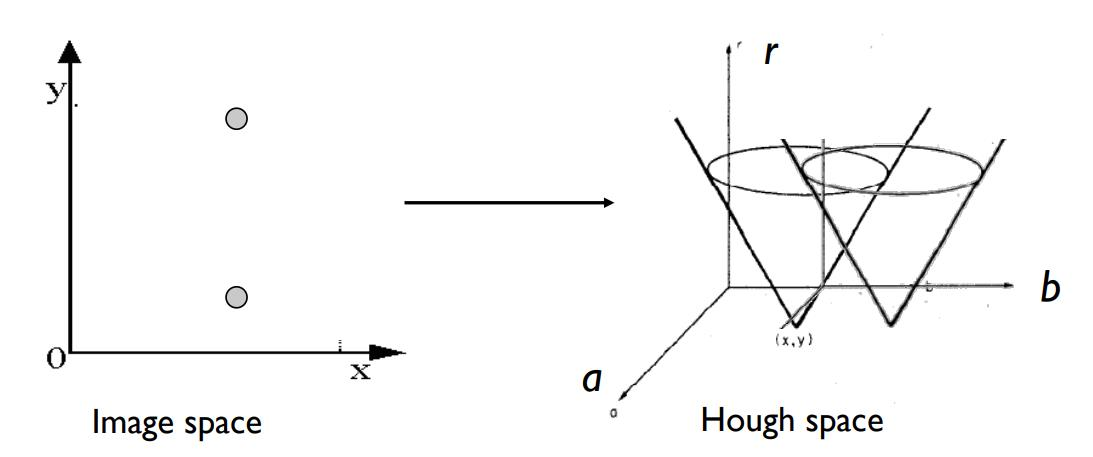
\includegraphics[width=0.7\linewidth]{img/hough_circle_accumulator_point}
\end{center}

\begin{equation*}
	y = a\cdot x + \sout{b}
\end{equation*}

\section{Semantic Segmentation}
Identify pixels in images belonging to a specific class, sometimes additionally identifying pixels to belong to a specific instance of a class. It can thus be understood as supervised learning at the pixel level.
\begin{center}
	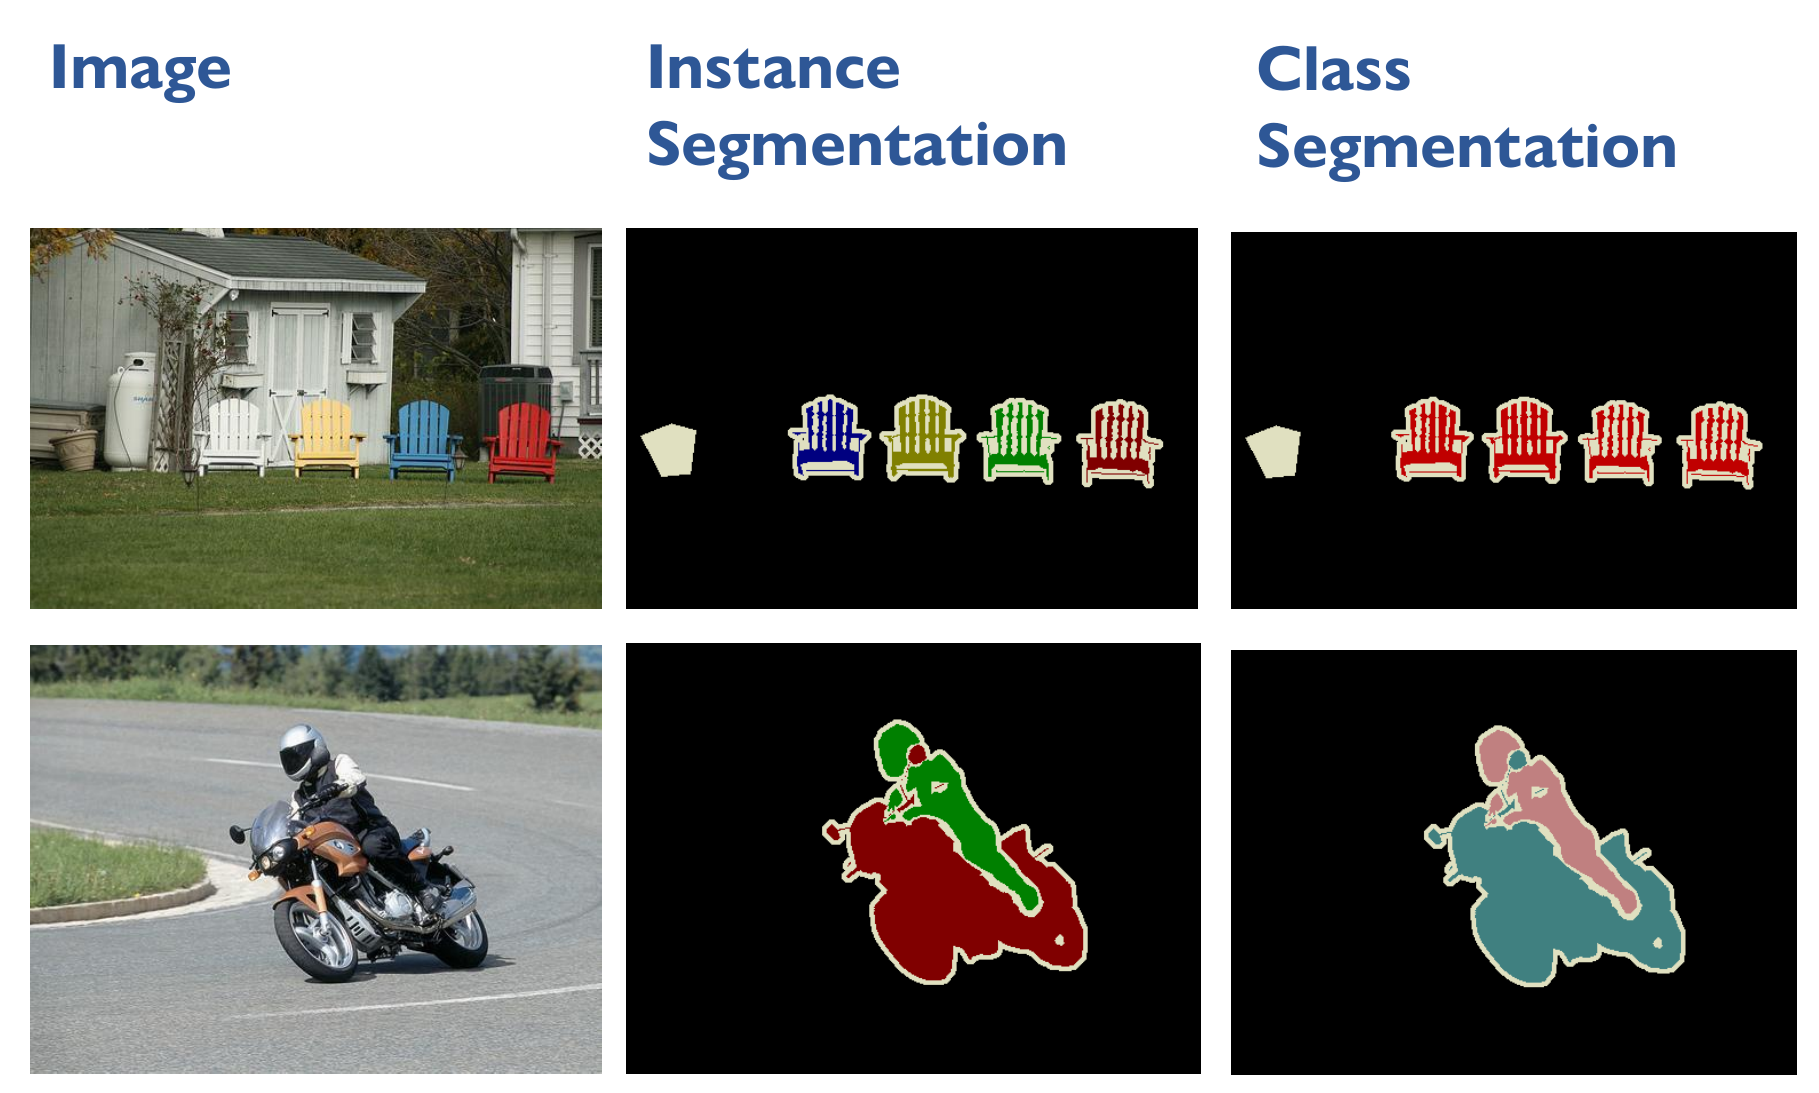
\includegraphics[width=0.7\linewidth]{img/semantic_segmentation}
\end{center}
Non-semantic segmentation tries to find regions in images without any additional information like classes or similar. It is thus similar to unsupervised learning and often a bottom-up approach. Segmentation in general tries to find a compact representation of a scene in terms of regions which share common properties.

\subsection{k-Means Clustering}
Is not an optimal solution to cluster an image. Lloyds algorithm is one possibility to do clustering
\begin{enumerate}
	\item[-] Initialise cluster centers (for example randomly)
	\item Calculate which samples belong to which clusters
	\item Calculate mean values of clusters as new centres
	\item[-] Iterate until clusters don't change
\end{enumerate}
Problems:
\begin{itemize}
	\item Number of clusters must be given
	\item Cluster shapes are given (spherical)
\end{itemize}

\subsection{Mean Shift Clustering}
The shape of the clusters should be variable and not be determined by the method. Mean shift clustering can be achieved by the algorithm
\begin{enumerate}
	\item Search for the maximum of the feature densitity from a given position in the image
	\item Define cluster as the set of positions that converge to the same maximum
\end{enumerate}
The problem to search for local maxima of the features without having a feature distribution available directly. The solution is to use a Kernel Density Estimation to describe the distribution, for example using the Gaussian kernel. Or using the Derivative of the Gaussian to get an approximation directly.
\begin{align*}
	\hat{f}_h(x) &= \frac{1}{nh}\sum_{i=1}^{n}K\left(\frac{x-x_i}{h}\right)\\
	K\left(\frac{x-x_i}{h}\right) &= \frac{1}{\sqrt{2\pi}} e^{-\frac{(x-x_i)^2}{2h^2}}
\end{align*}
\begin{center}
	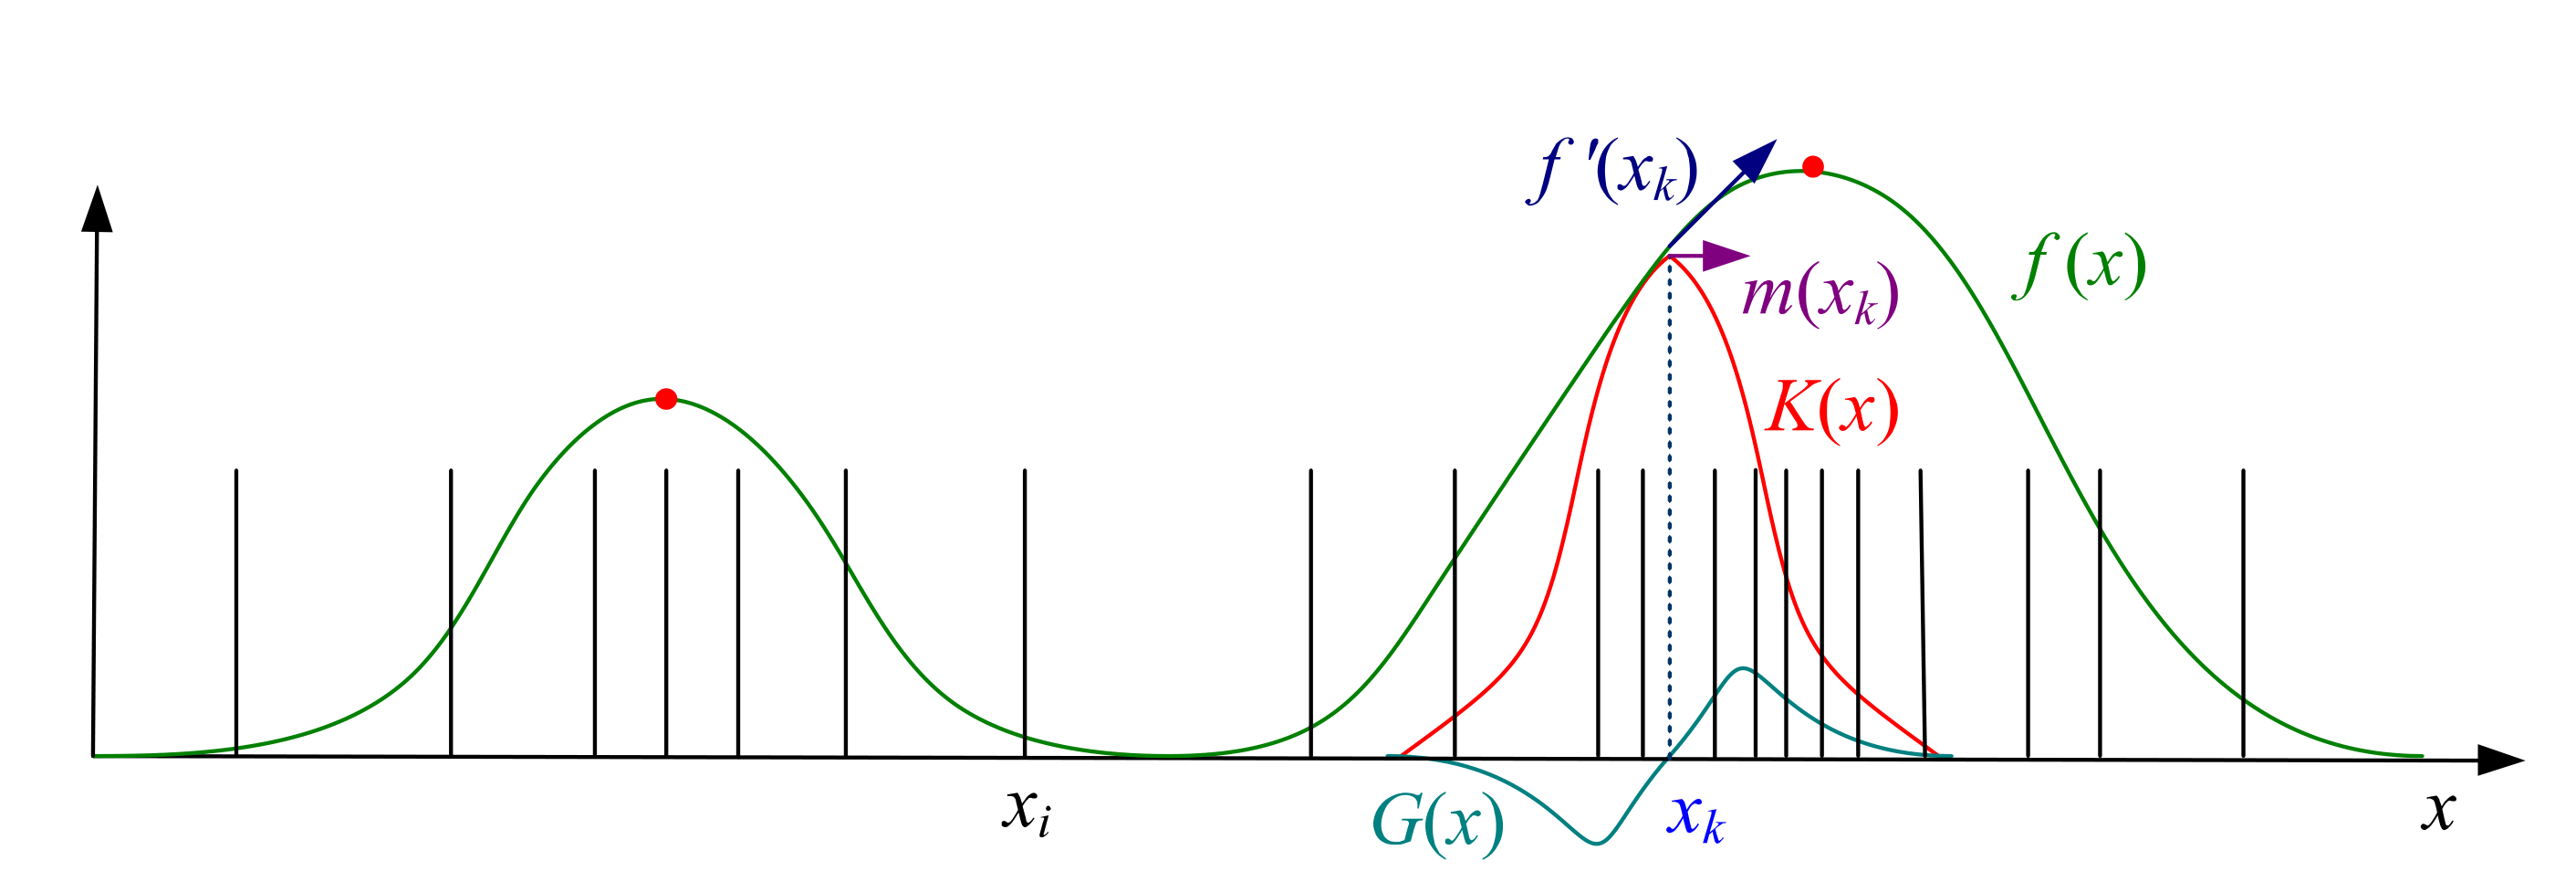
\includegraphics[width=0.7\linewidth]{img/kernel_density_estimation}
\end{center}

\subsubsection{Mean Shift Algorithm}
\begin{itemize}[label=-]
	\item[] For all positions $x$ in the image
	\item Calculate the mean $\samplemean{x}$ in the environment $N(x)$
	\begin{equation*}
		\samplemean{x} = \frac{\sum_{x_i \in N(x)} K(x_i - x) x_i }{\sum_{x_i \in N(x)} K(x_i - x)}
	\end{equation*}
	\item Set $x$ to the mean $\samplemean{x}$
	\item Iterate until $x$ does not change
\end{itemize}
Attraction basins are regions from which all trajectories lead to the same node.
\begin{center}
	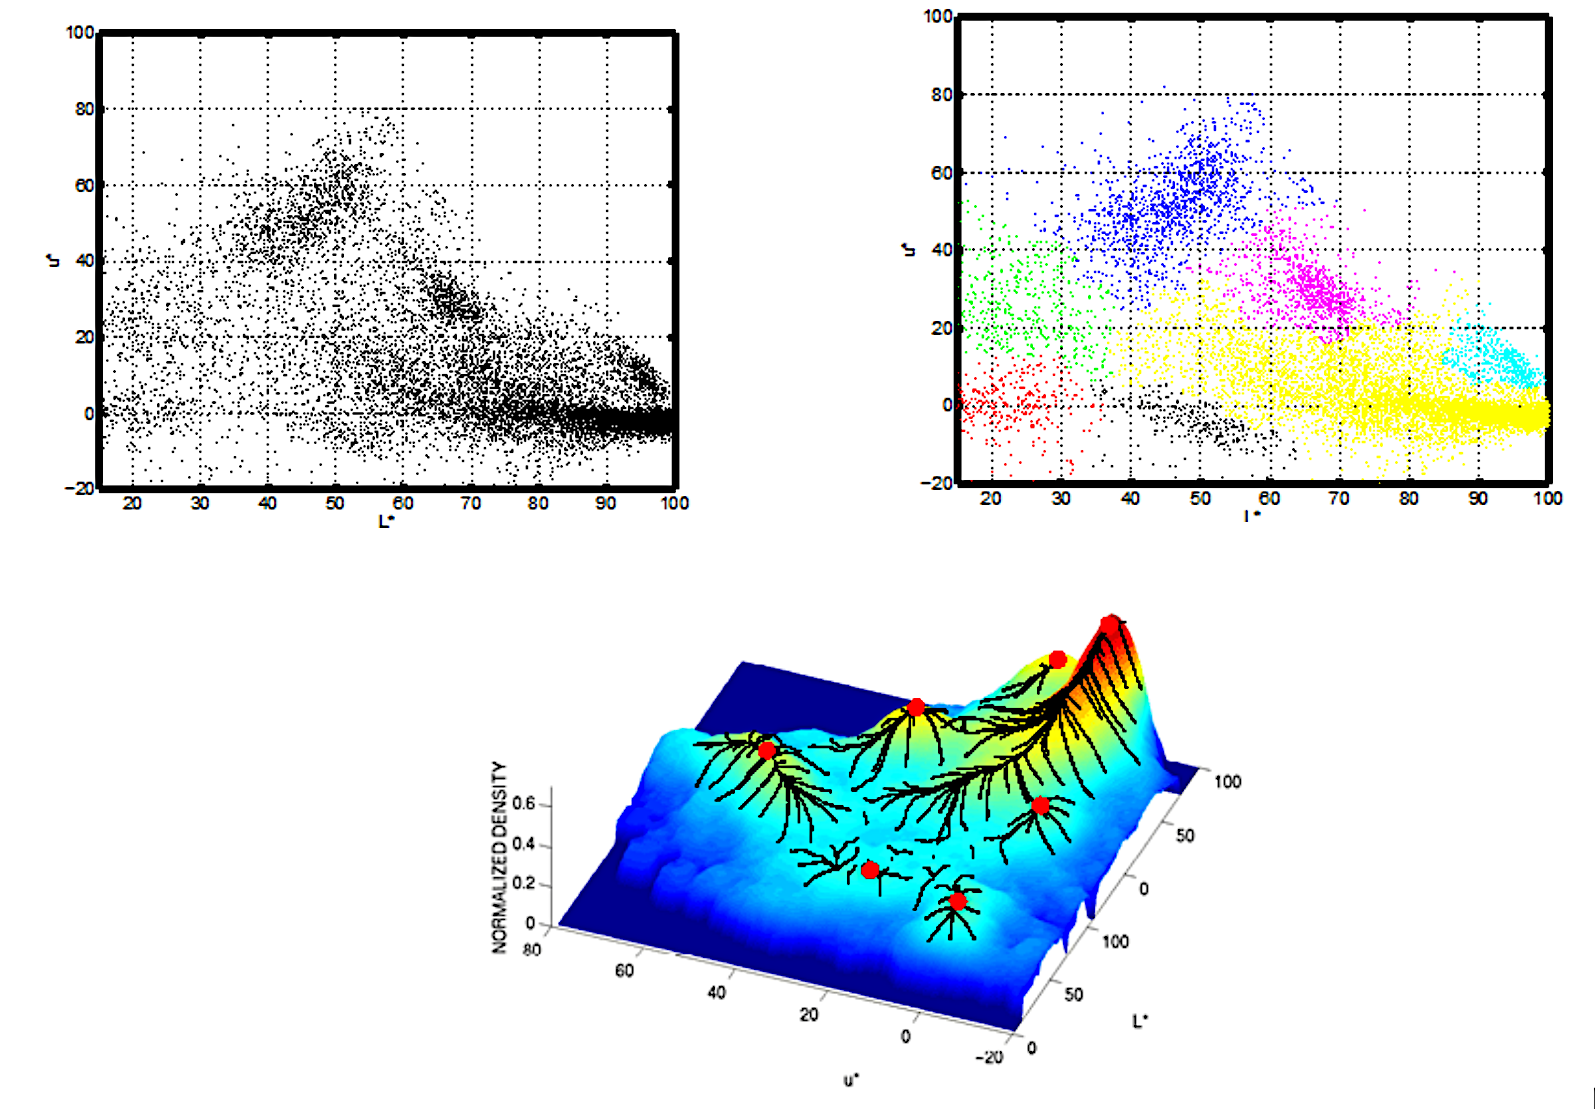
\includegraphics[width=0.7\linewidth]{img/attraction_basins}
\end{center}

\subsection{Segmentation by Graph Cuts}
Images are seen as graph with a node for every pixel with edges between nodes with an affinity weight for each edge. This weight  measures similarity, for example inversely proportional to difference in colour and position.
\begin{definition}
	Let $G=(V,E)$ be a graph. Each edge $(u,v)$ has a weight $w(u,v)$ that represents the similarity between $u$ and $v$. Cut $G$ into two disjoint graphs with node sets $A$ and $B$ by removing all edges between those sets. Assign a value to the cut as follows
	\begin{equation*}
		\text{cut}(A,B) = \sum_{u\in A,v\in B}^{w(u,v)}
	\end{equation*}
\end{definition}
Minimal value cuts often cuts too small groups. A better approach is to use normalised cuts:
\begin{align*}
	\text{Ncut}(A,B) &= \frac{\text{cut}(A,B)}{\text{assoc}(A,V)} + \frac{\text{cut}(A,B)}{\text{assoc}(B,V)}\\
	\text{assoc}(A,V) &= \sum_{u\in A, t\in V}^{w(u,t)}
\end{align*}
where $V$ is the set of all vertices.

\subsection{Superpixels}
The problem is that images contain many pixels and it is thus inefficient for graph calculations. The solution is to calculate \emph{superpixels} by grouping similar pixels first. This is cheap but leads to over-segmentation. As soon as the superpixels are calculated, normalised graph cuts can be applied.

\subsection{Features}
Usually, Raw Input pixel values are not used as input features, as this makes the input space to big. Instead a feature vector is calculated for each pixel or set of pixels. These feature calculate certain properties of an image or image region. Besides classification tasks, these vectors are also used to find subregion or image stitching, and more.

\subsubsection{Feature Properties}
Features should be invariant to
\begin{itemize}[label=-]
	\item Translation
	\item Rotation
	\item Scaling
	\item Illumination, color changes
	\item Transformation (Skewing)
\end{itemize}

\subsubsection{Filter Banks}
\begin{center}
	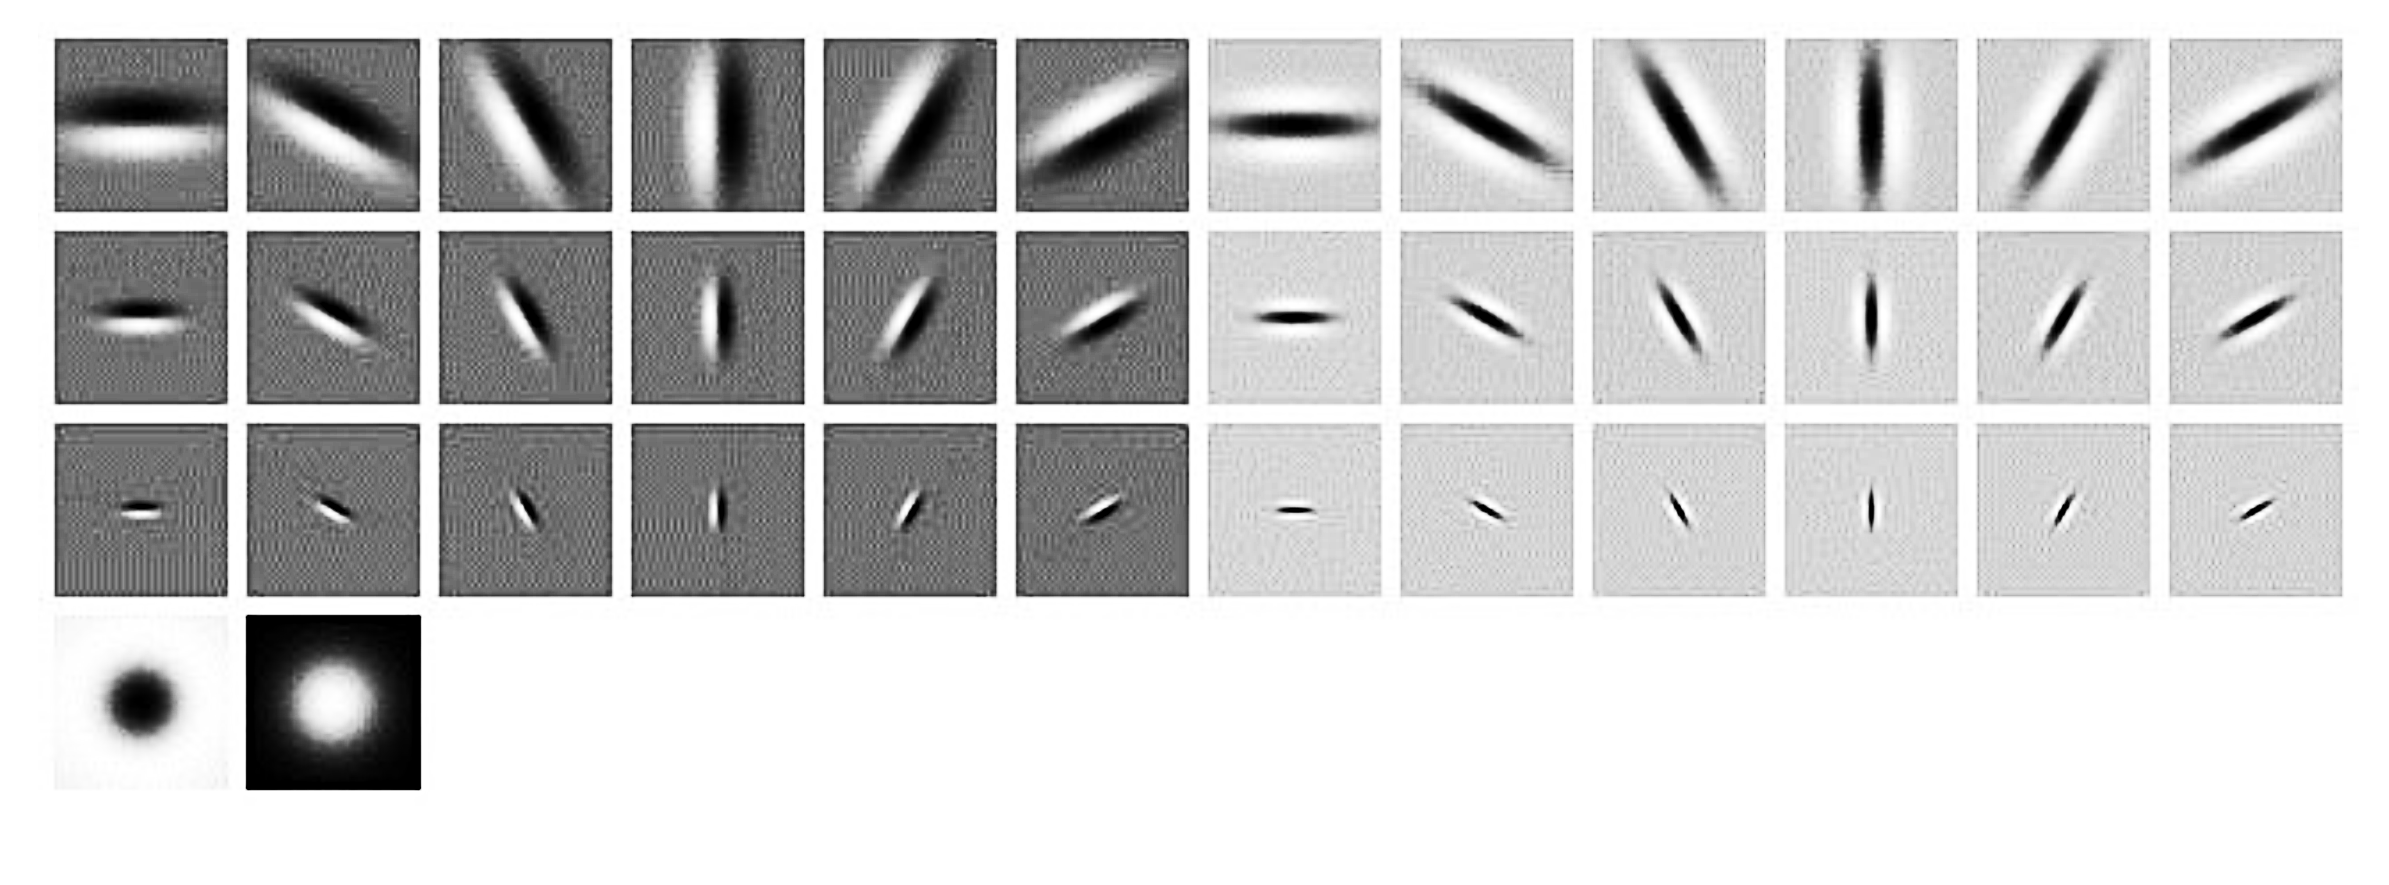
\includegraphics[width=0.6\linewidth]{img/filter_bank}
\end{center}
\begin{itemize}
	\item RFS Filters: edge and line filters at six orientations and three scales, Gaussian and Laplacian of Gaussian
	\item MR8 Filters: Maxima of RFS Filters at each scale
\end{itemize}

\subsubsection{Texture Characteristics}
Textons use the texture descriptor as vectors of filter bank outputs. Textons found by clustering are called a dictionary generation. For comparison, use the similarity between regions in the Texton histograms directly.

\subsubsection{Grey Level Co-occurence Matrices (GLCMs)}
Measurement of how often a specific combination of a colour value between a pixel and its neighbours occur. This results in a $256\times 256$ matrix for the 256 grey values. Additional features like entropy, energy, homogeneity, contrast or dissimilarity can be calculated from the matrix.

\subsubsection{Scale Invariant Feature Transform (SIFT)}
Popular feature descriptor for various tasks such as object matching, image stitching and more. It is a combination of detector and descriptor. The descriptor uses the histogram of the gradient. SIFT results in a 128-dimensional vector.
\begin{center}
	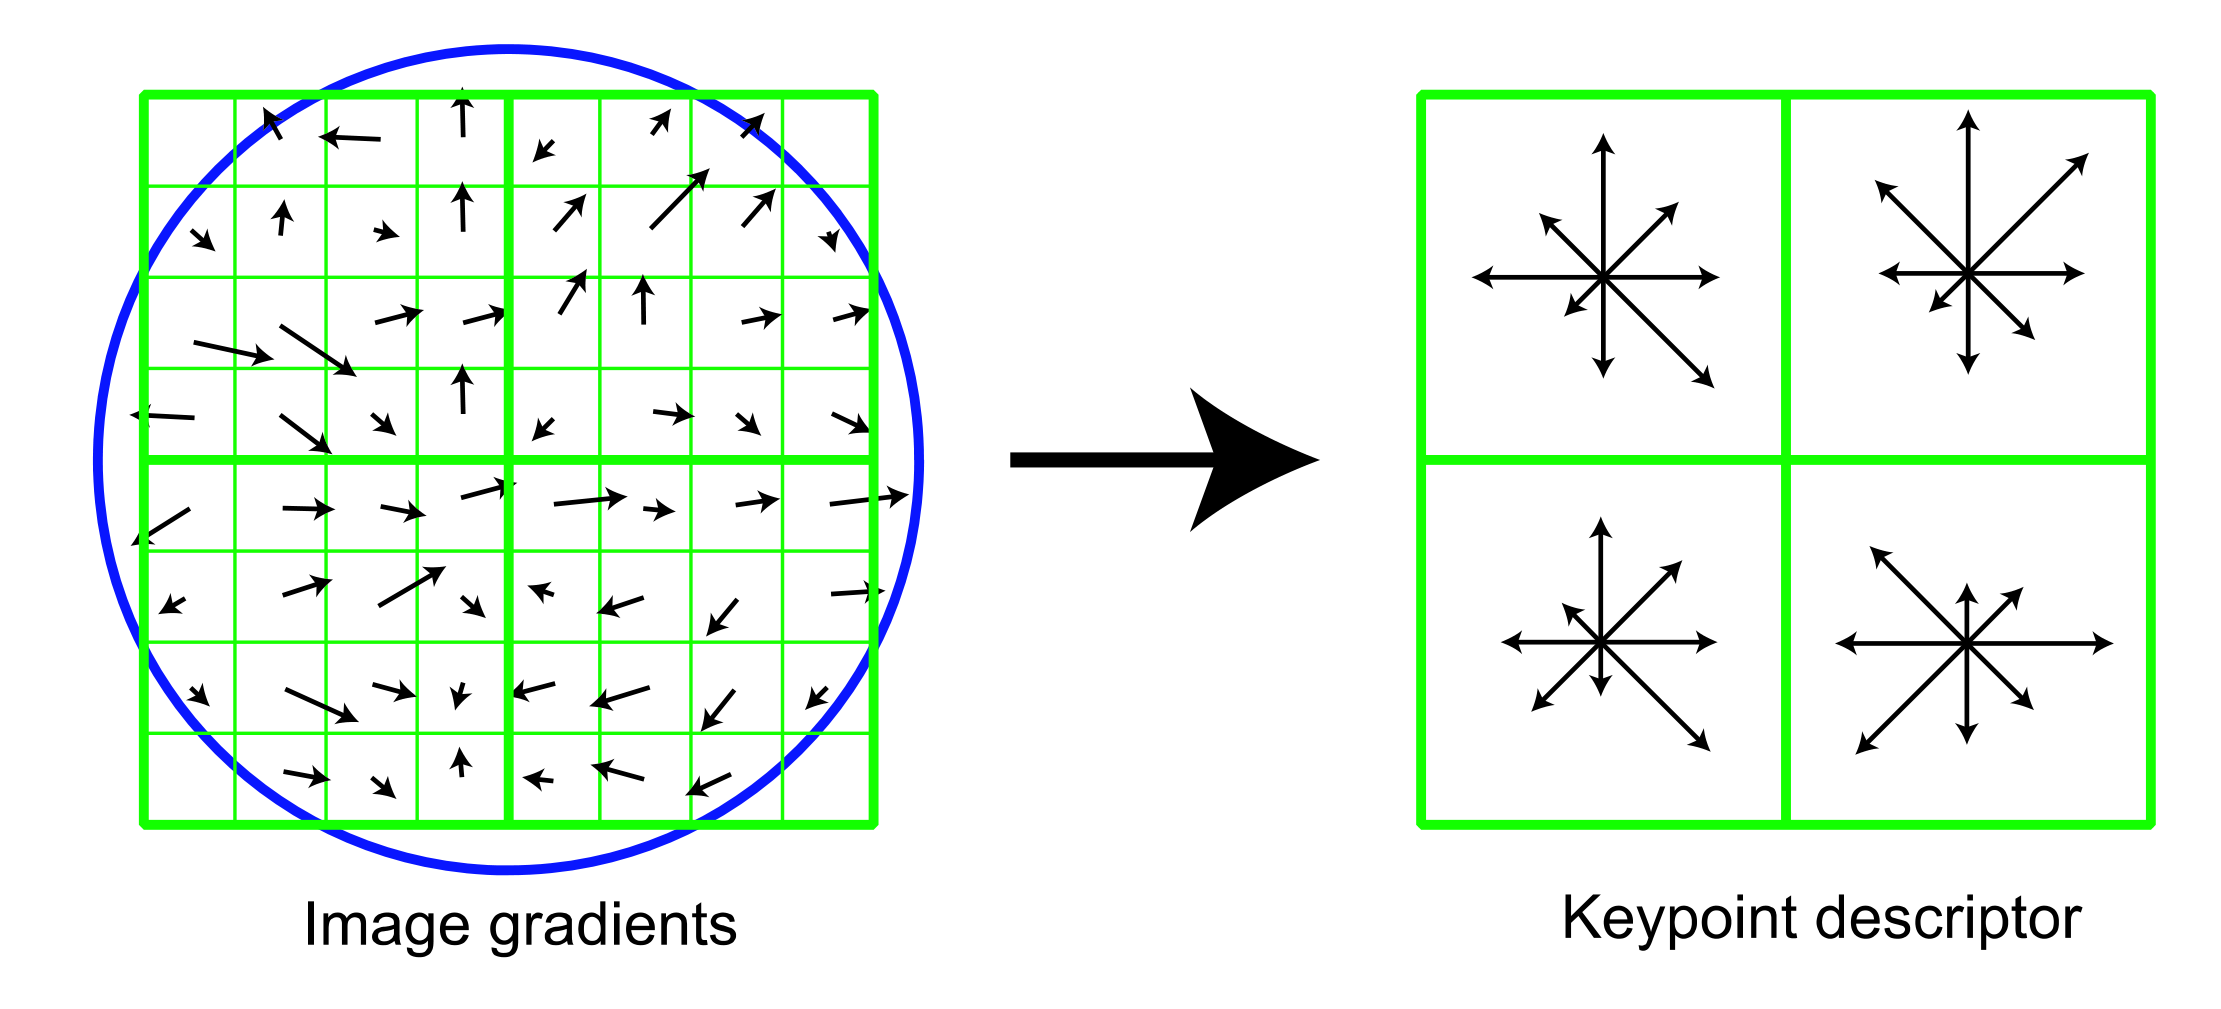
\includegraphics[width=0.6\linewidth]{img/SIFT}
\end{center}

\subsubsection{Histogram of Oriented Gradients (HOG)}
Computes the gradient images in x and y, and divides the image into cells. Compute histogram of gradient orientation in cell, normalise and flatten it into a feature vector.

\subsubsection{HOGles}
"Invert" the HOG features to simulate the image that generates it. This is a helpful tool to understand bad detections.

\begin{center}
	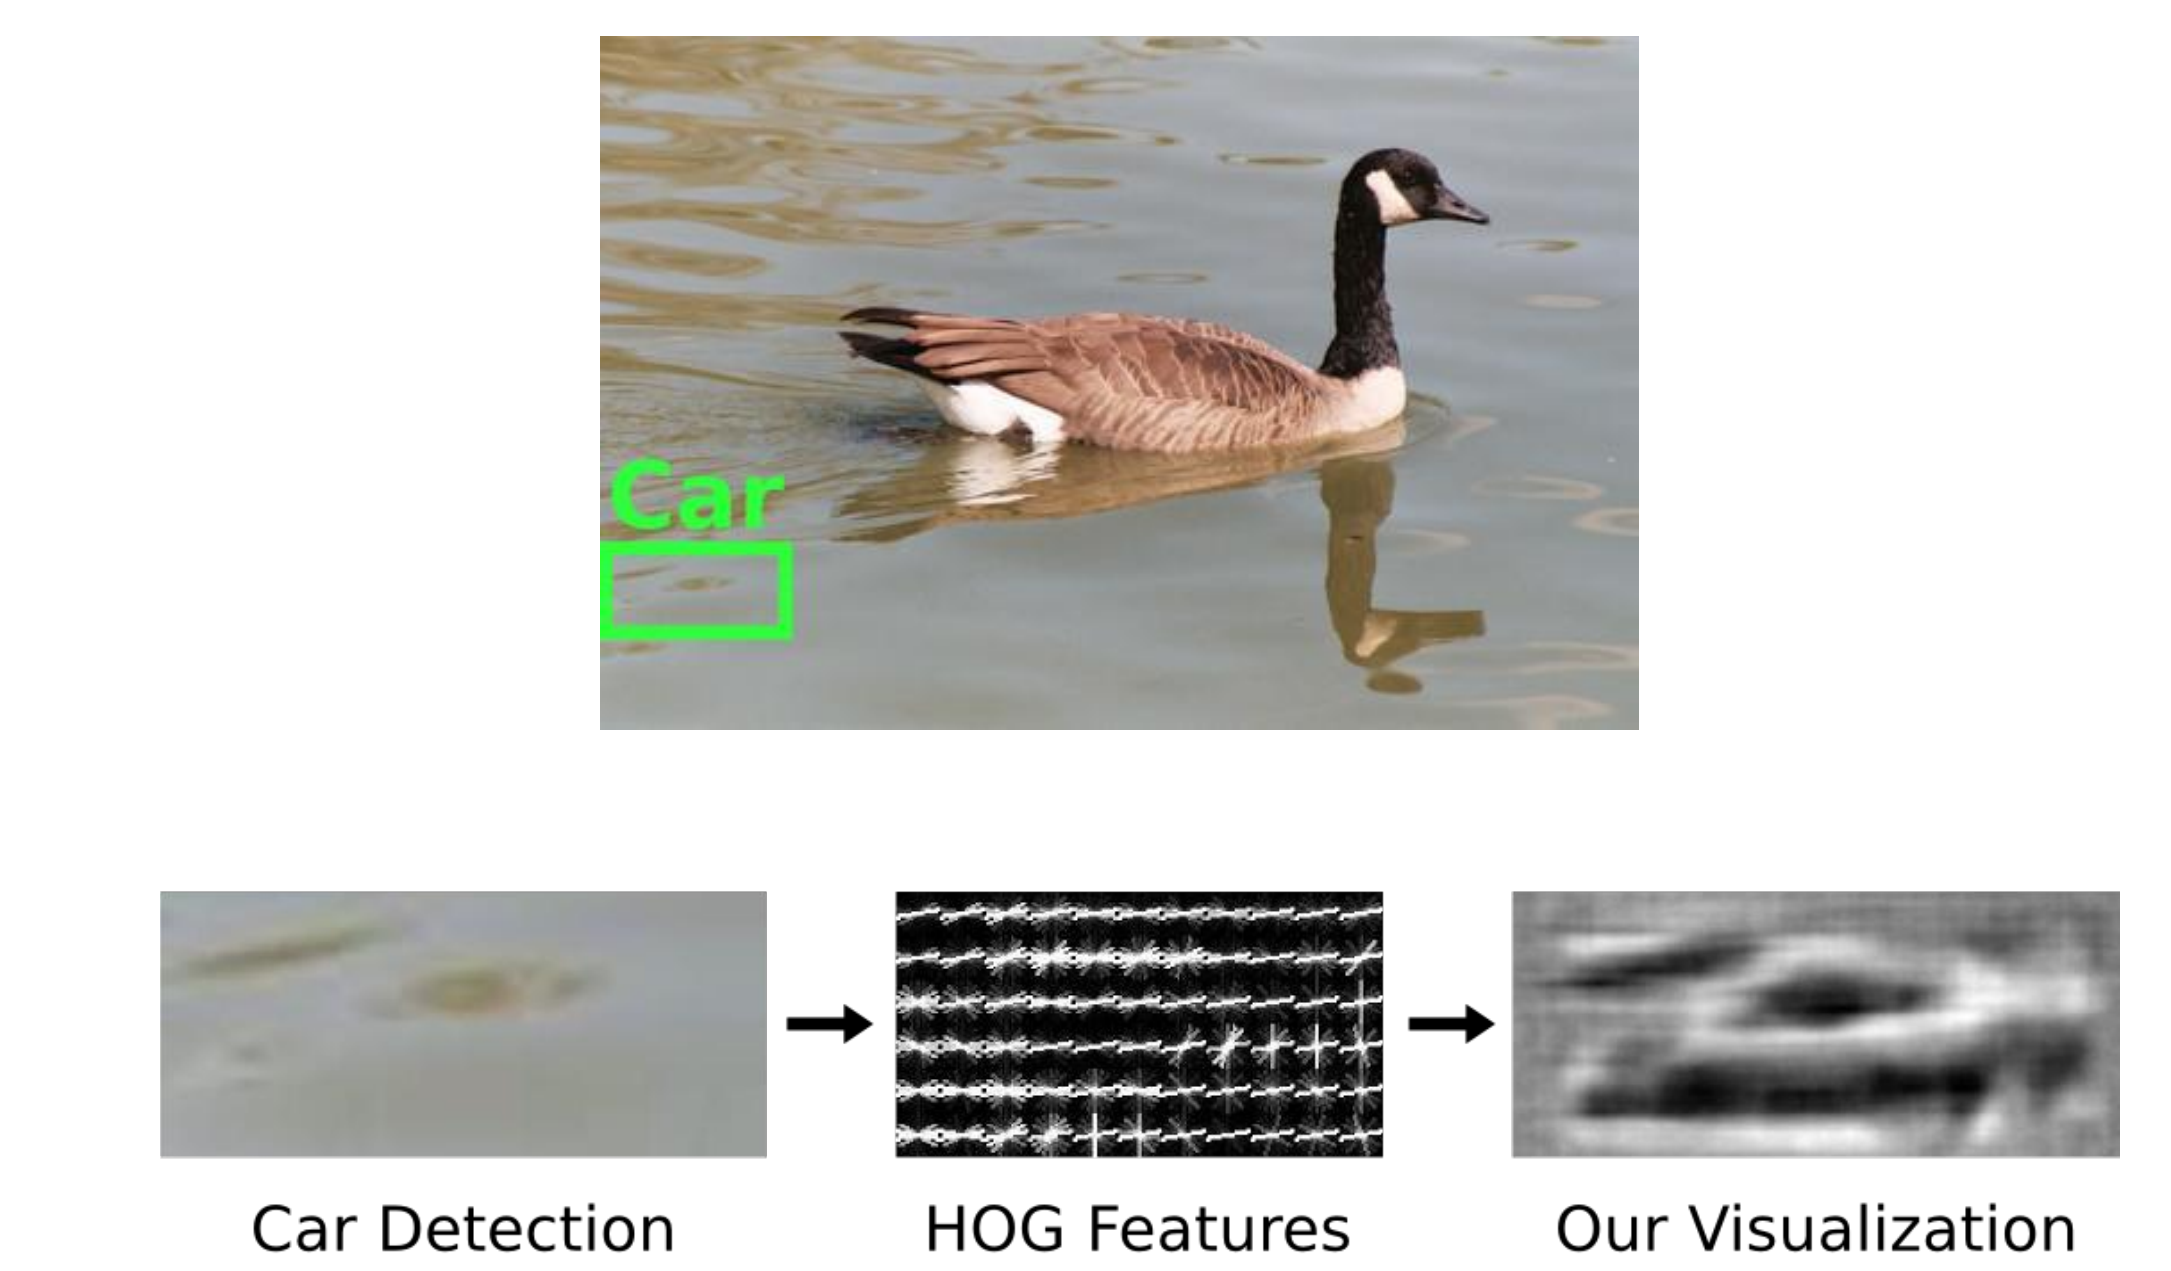
\includegraphics[width=0.6\linewidth]{img/HOGles}
\end{center}

\section{Finding Multiple Objects}
The problem at the core is how to scan many positions efficiently for possible faces. Possible approaches are
\begin{itemize}[label=-, nosep]
	\item {\color{DodgerBlue4} Features}
	\item {\color{DodgerBlue4} Classifier}
	\item {\color{DodgerBlue4} Sliding Window}
	\item {\color{Firebrick1} Haar Features}
	\item {\color{Firebrick1} Boosting}
	\item {\color{Firebrick1} Cascaded Classifiers}
\end{itemize}

\subsection{Boosting}
For an input training data with weights, at each step $t \in 1..T$ train a weak classifier, let it classify the training data and increase the weight on incorrectly classified samples. Use the weighted combination of all weak classifiers for the final, strong classifier. The final strong classifier $F(x)$ can be understood as a weighted, linear combination of the weak classifiers.
\begin{equation*}
	F(x) = \alpha_1 f_1(x) + \alpha_2 f_2(x) + \alpha_2 f_2(x) + \dots
\end{equation*}
Weak classifier used with $f$ feature, $\theta$ threshold and $p_j$ parity
\begin{equation*}
	h_j (\theta) = \left\{ \begin{matrix}
		1 & p_j f_j < p_j \theta_j\\
		0 & \text{otherwise}
		\end{matrix} \right.
\end{equation*}

\subsection{Haar Features}
Filter responses, that is convolutions, are computationally intensive. The idea of haar features is to only use simple filters of different sizes and shapes with only $-1$ or $1$ in the masks. Calculate the features on sliding sub windows (for example $24\times24$ pixels) and take all possible combinations of filters as feature candidates. This can be done in a fast manner using integral images, where each pixel of the integral image contains the sum of all values in the rectangle spanned to the upper left corner (see image \ref{fig:integralimage}). The sum of pixel $D$ in figure \ref{fig:integralimagehaar} is $4 + 1 - (2 + 3)$ or in terms of the named rectangles
\begin{equation*}
	D = (A+B+C+D) + A - ((A+B) + (A+C))
\end{equation*}

\begin{figure}[tbh]
	\centering
	\begin{subfigure}[t]{0.45\linewidth}
		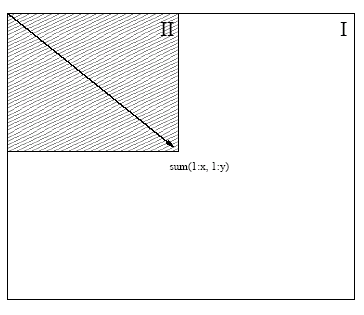
\includegraphics[width=\linewidth]{img/integral_image}
		\caption{Visualisation of an integral image sum}
		\label{fig:integralimage}
	\end{subfigure}
	\begin{subfigure}[t]{0.45\linewidth}
	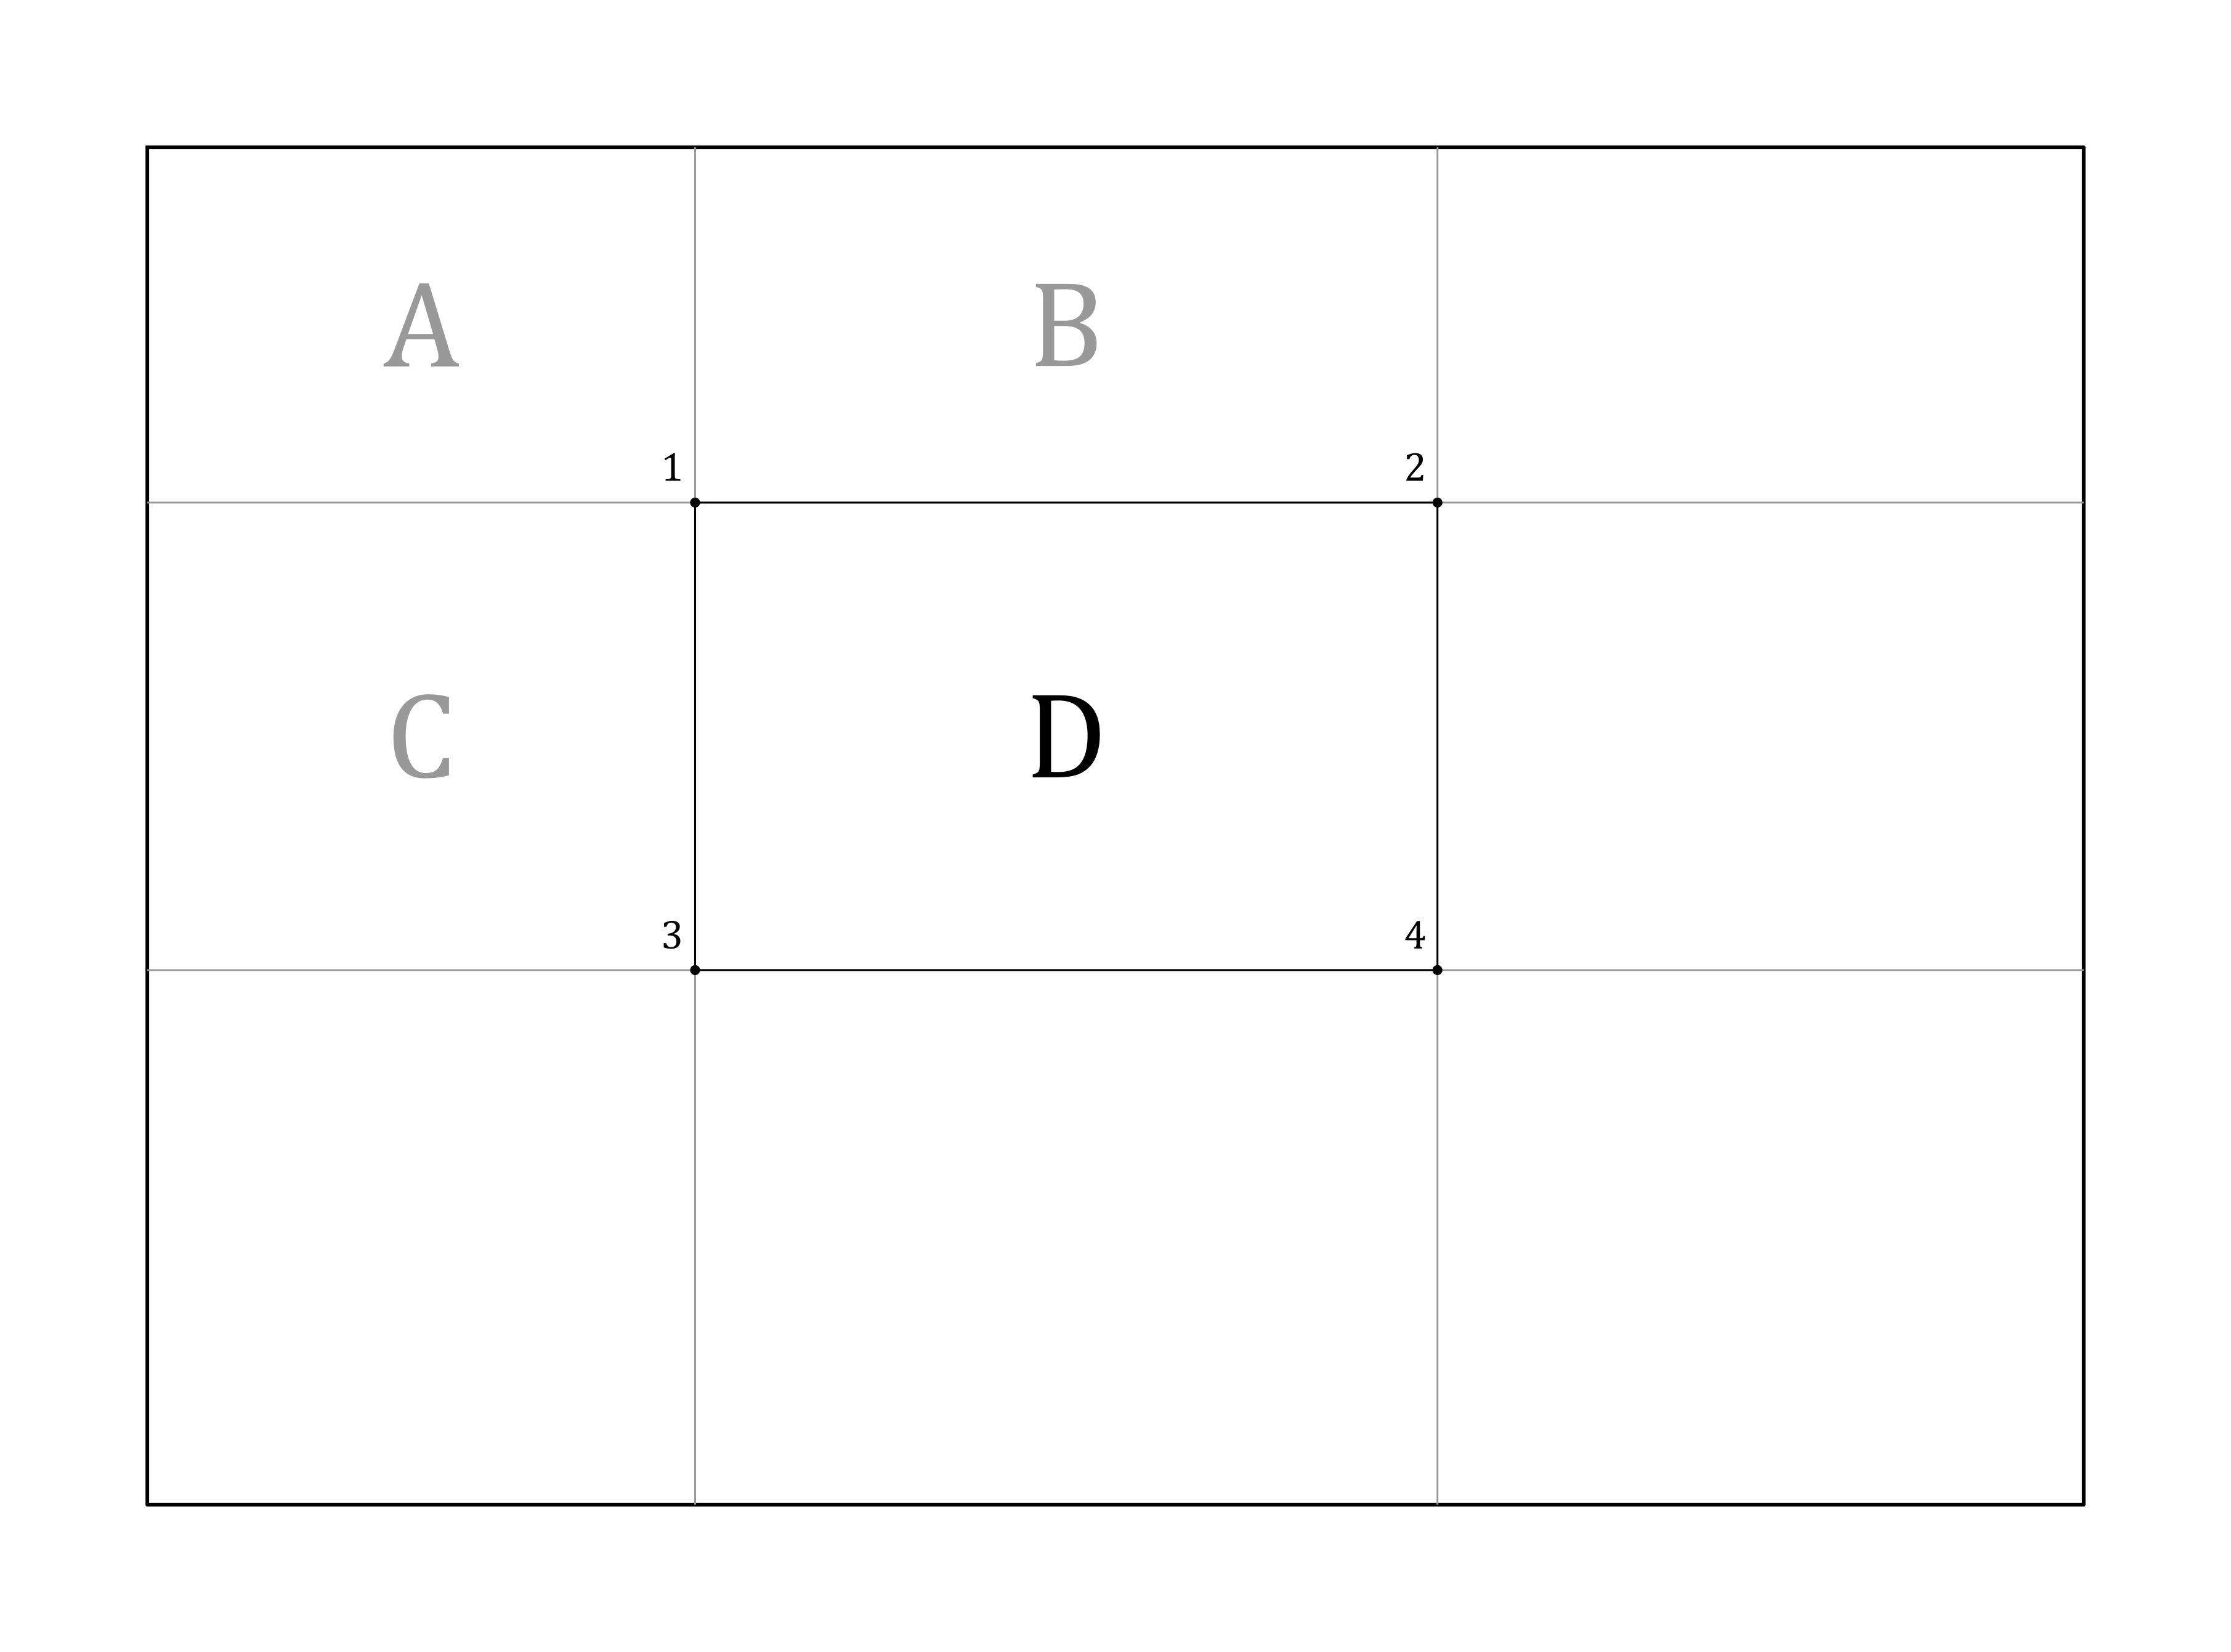
\includegraphics[width=\linewidth]{img/integral_image_haar}
	\caption{Calculating Haar features using an integral image}
	\label{fig:integralimagehaar}
	\end{subfigure}
\end{figure}
The humongous size of the features per sub window can be evaluated by treating each feature as a weak classifier and training important features using adaboost.

\subsection{Face Detection}
The problem is that there are thousands of possible position or scale combinations in the image which need to be evaluated, while true faces are rare in the image. The idea is thus to dismiss the regions without a face efficiently. The goal for a classifier is to have a high \emph{true} positive rate (85\%-95\%) and a low \emph{false} positive rate ($10^{-5}-10^{-6}$). Use this classifier in a cascade which multiplies false and true positive rates. False results are rejected early in the processing.
\begin{center}
	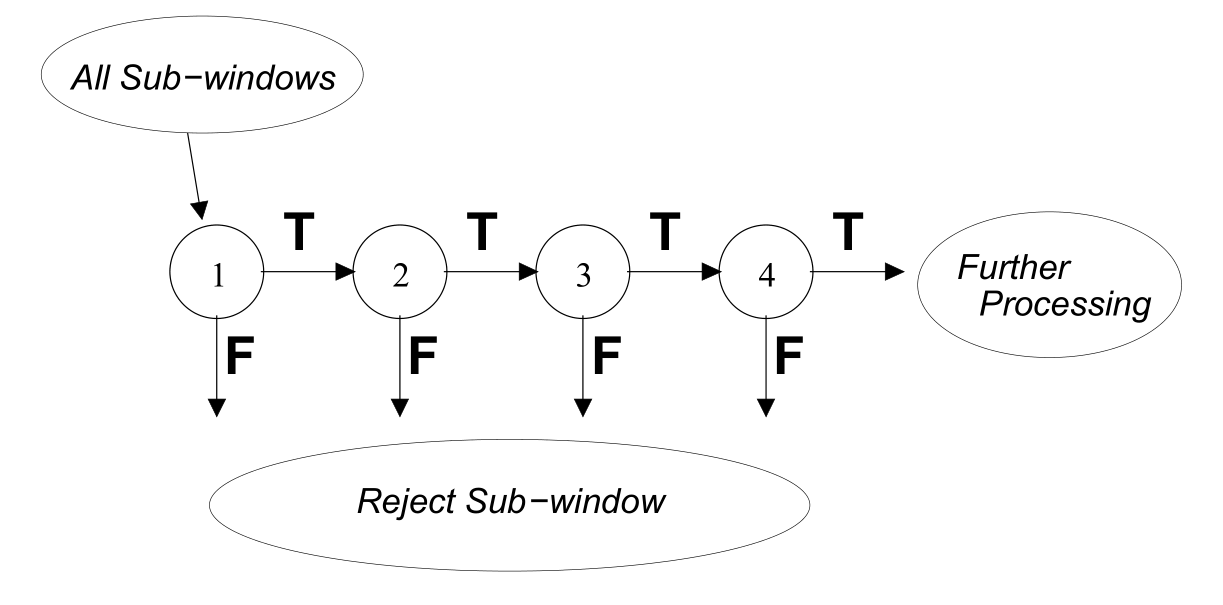
\includegraphics[width=0.6\linewidth]{img/cascade_classifier_approach}
\end{center}

\subsection{HOG for Human Detection}
Detection Pipeline
\begin{itemize}[label=-]
	\item Calculate HOG Descriptors
	\item Collect HOGs in Detection Window
	\item Use Linear SVM for Person or Non-Person Classification
\end{itemize}
\begin{center}
	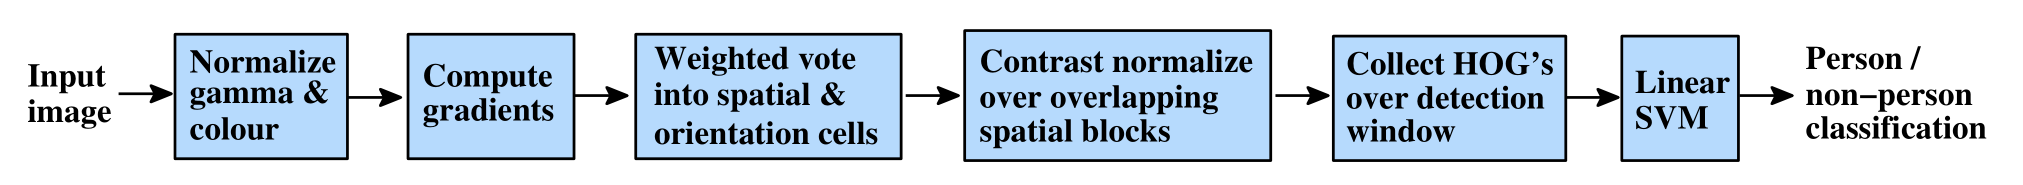
\includegraphics[width=0.8\linewidth]{img/hog_human_detection}
\end{center}

\subsection{OverFeat}
Combine Classification, Localisation and Detection.
\begin{itemize}[label=]
	\item Classification
	\begin{itemize}[label=-,nosep]
		\item CNN
		\item Sliding Windows, apply at every possible pixel and at multiple scales
		\item Subsampling factor of 12
	\end{itemize}
	\item Localisation
	\begin{itemize}[label=-,nosep]
		\item Generate Bounding Box Prediction, as a Regression Problem
		\item Uses the same first five layers in the CNN
	\end{itemize}
	\item Detection
	\begin{itemize}[label=-,nosep]
		\item Combine Classification and Localisation
		\item Merge and accumulate bounding boxes
	\end{itemize}
\end{itemize}

\begin{figure}[tbh]
	\centering
	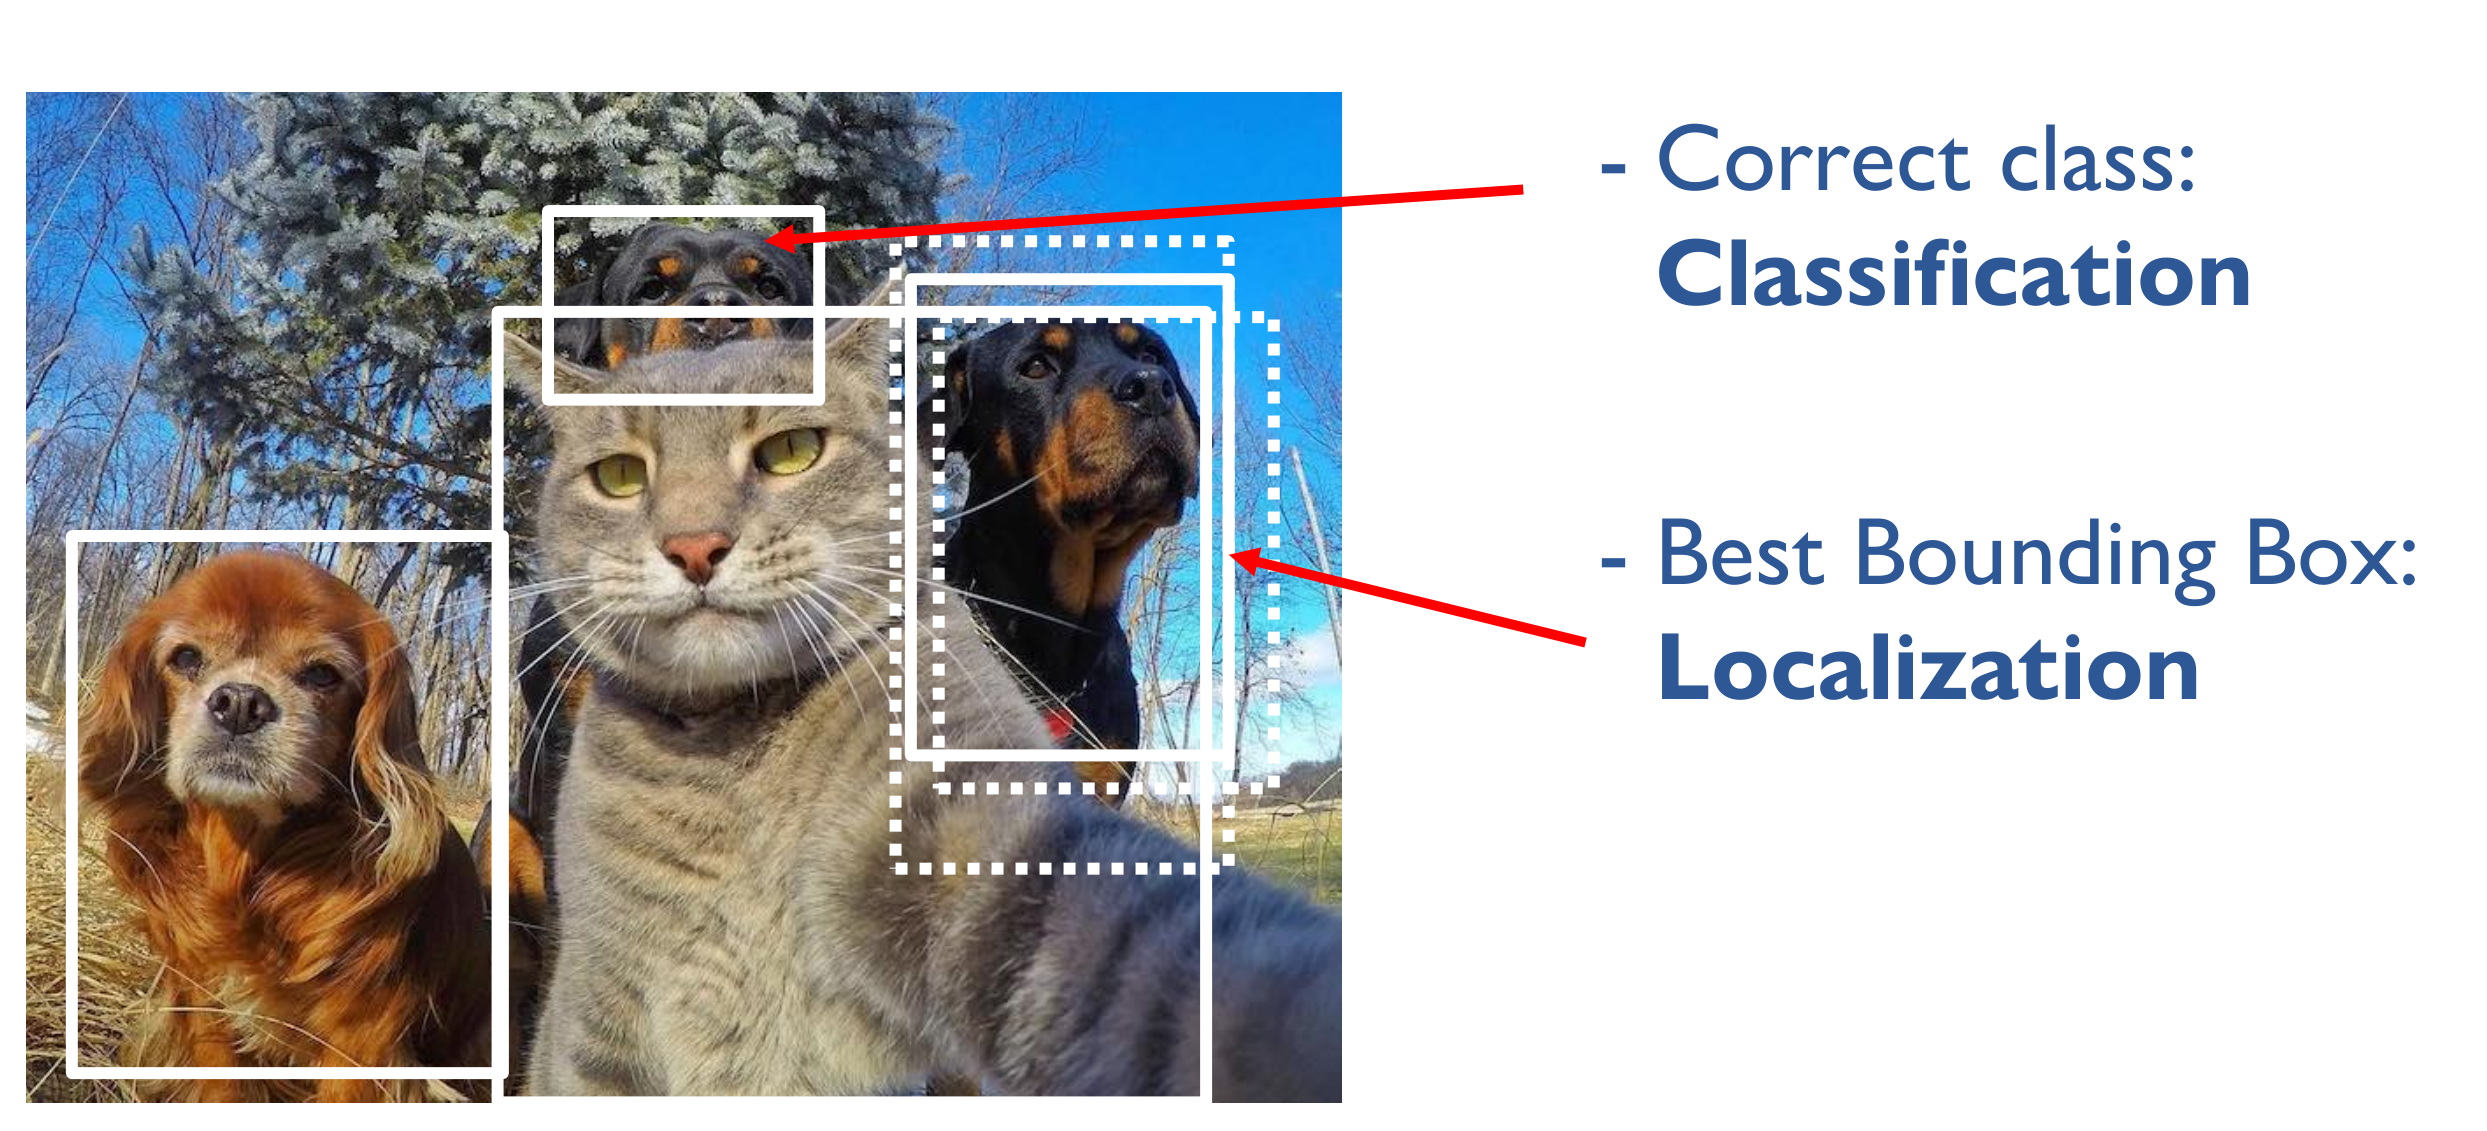
\includegraphics[width=0.7\linewidth]{img/classification_localisation}
	\caption{Classification and Localisation visualised}
	\label{fig:classificationlocalisation}
\end{figure}

Sliding windows have the drawback of the huge numbers of different positions and sizes that need to be evaluated. A better idea would be to find image regions that are likely to contain an object, which are called region proposals.

\subsection{R-CNN}
Extract region proposals, compute CNN features on these, classify the regions using SVM.
\begin{center}
	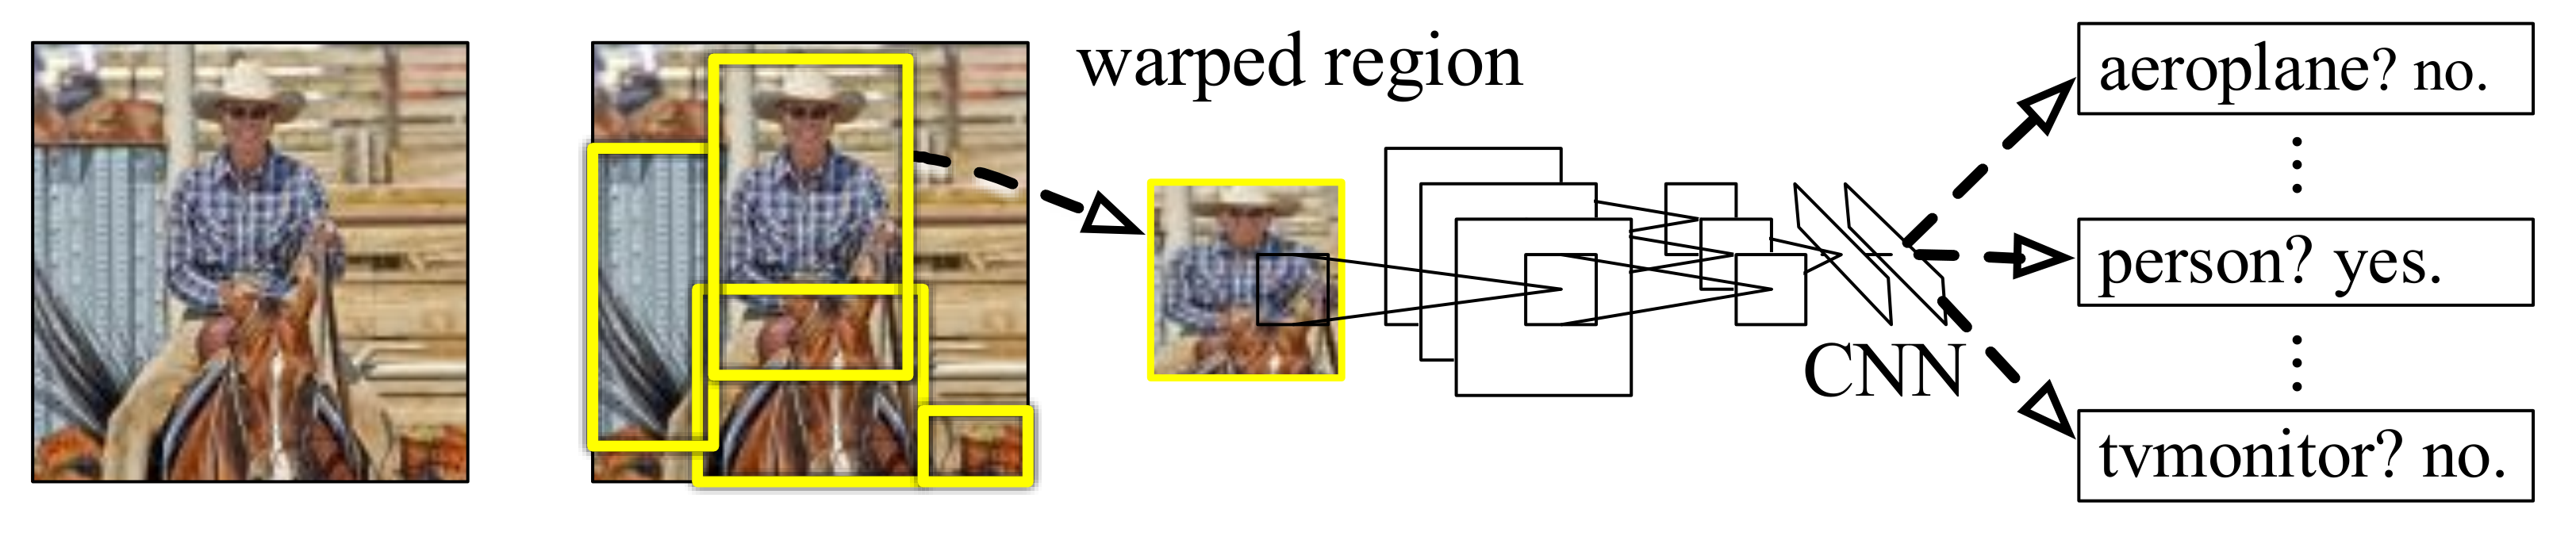
\includegraphics[width=0.7\linewidth]{img/r-cnn}
\end{center}

\begin{center}
	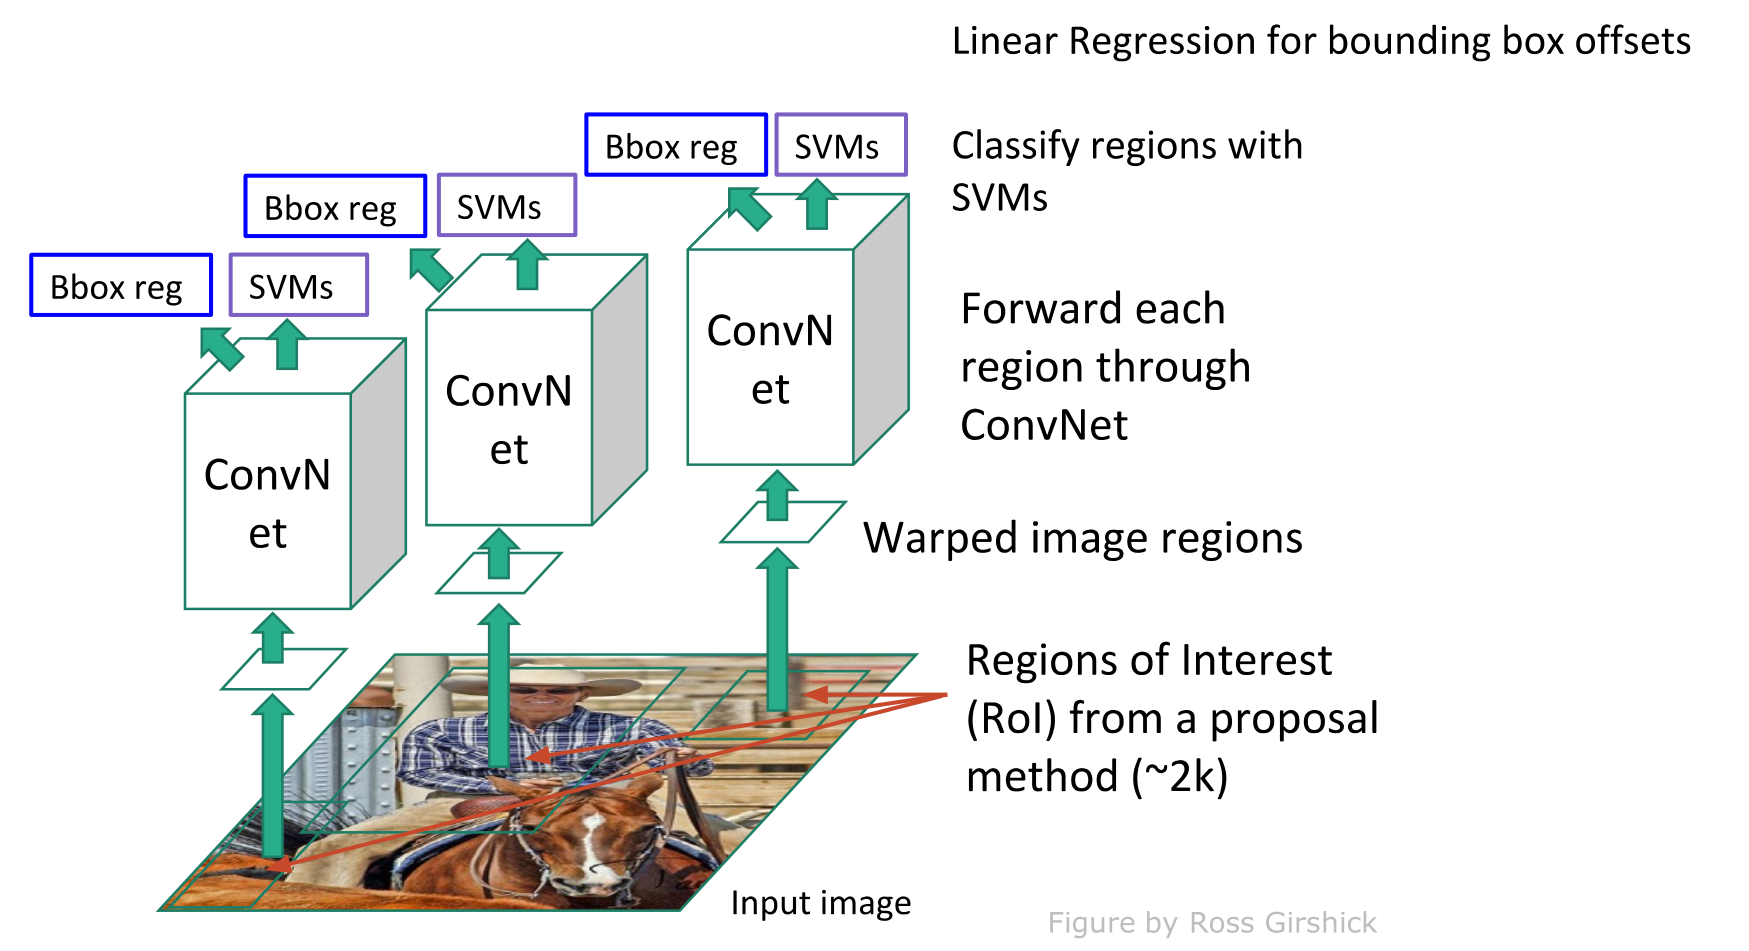
\includegraphics[width=0.7\linewidth]{img/r-cnn_structure}
\end{center}

\subsubsection{Feature Extraction}
\begin{itemize}
	\item Proposal regions are warped to $227\times 227$ pixel images
	\item 4096 Features from $227\times 227$ RGB Image using five Convolutional and two fully connected layers from AlexNet Architecture
	\item Supervised pre-training on the ILSVRC2012 classification data set
	\item Domain-specific fine-tuning is done by continuing training on warped region proposals
\end{itemize}

\subsubsection{Classifier}
Use one linear SVM per class (one true class versus all others), consider regions with overlap of 30\% a positive example and treat the bounding box position as regression problem.

\subsubsection{FAST R-CNN}
Replace SVM of R-CNN with fully connected neural network for classification of objects and refined bounding boxes
\begin{center}
	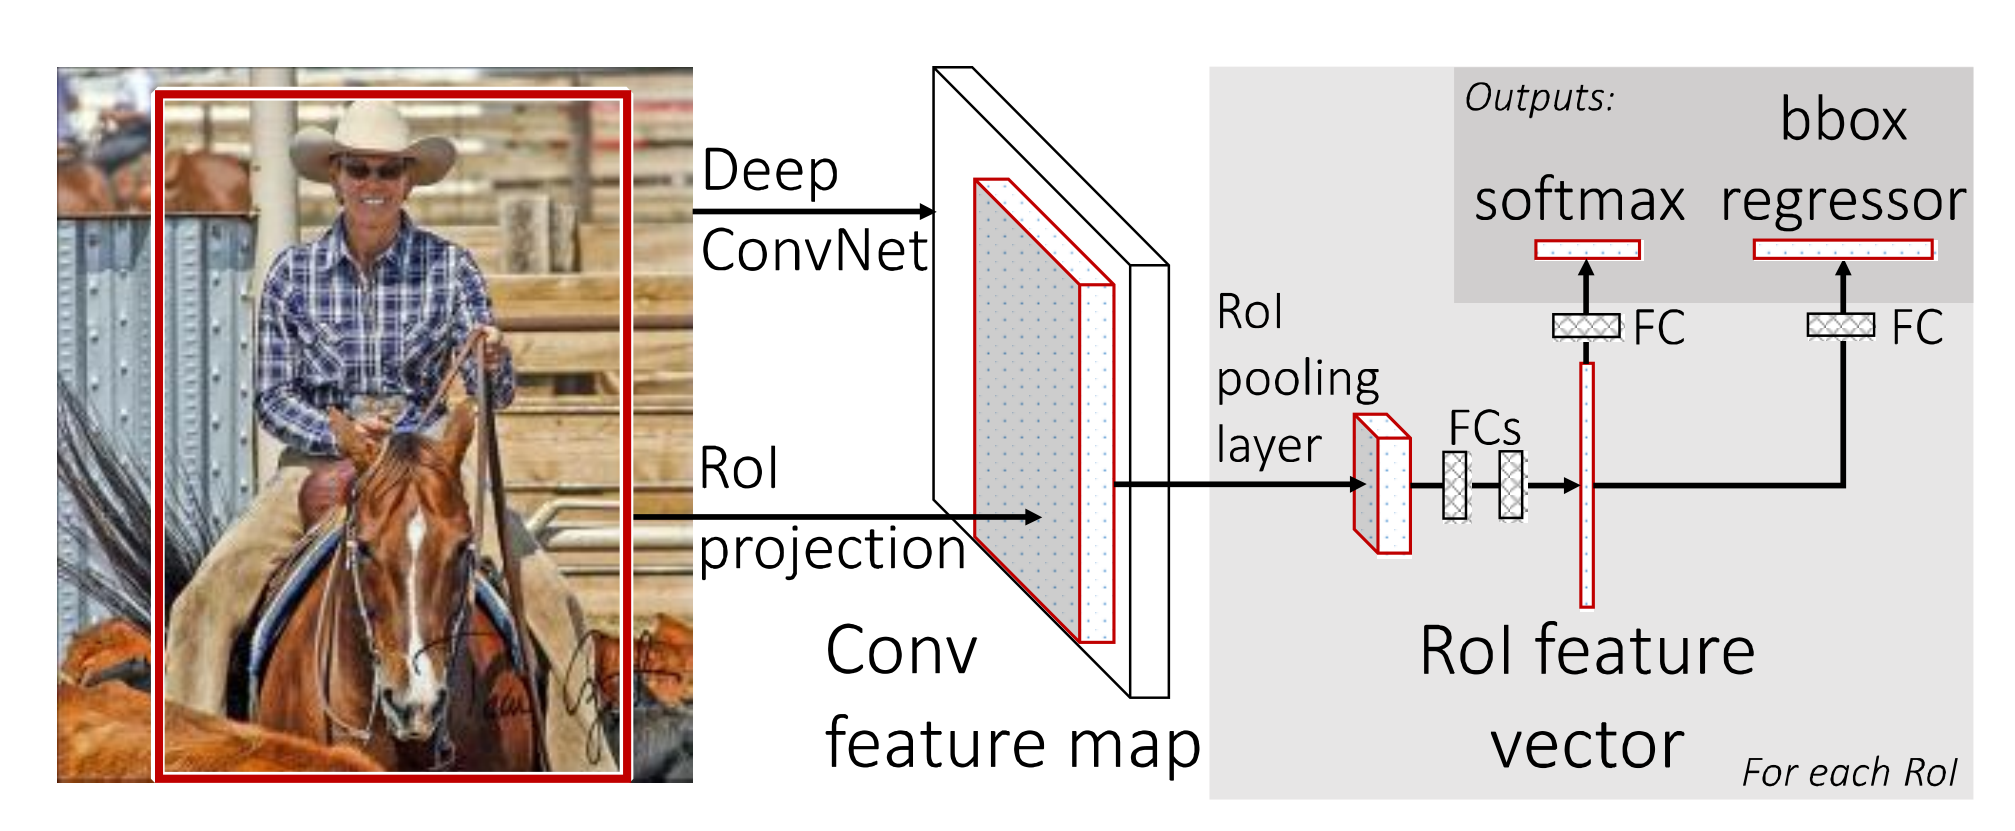
\includegraphics[width=0.7\linewidth]{img/fast_r-cnn_structure}
	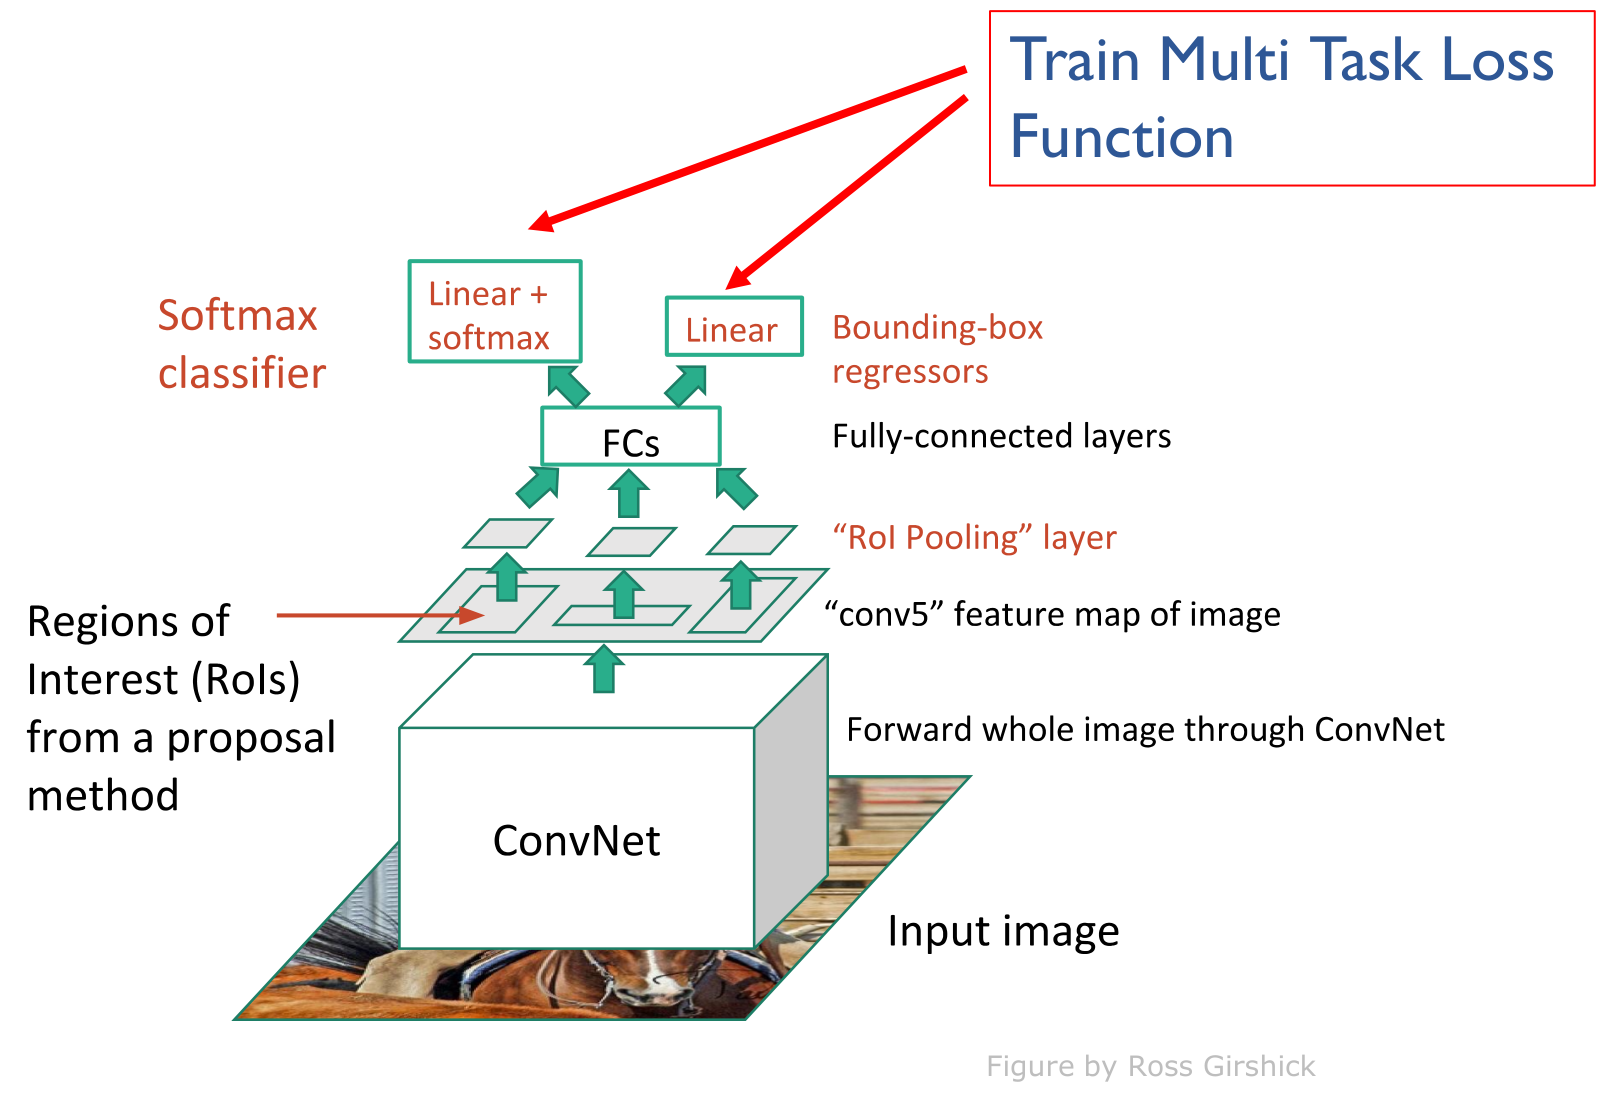
\includegraphics[width=0.7\linewidth]{img/fast_r-cnn_structure2}
\end{center}

\subsection{You Only Look Once (YOLO)}
YOLO is a Single Neural Network that predicts bounding boxes and classification probabilities, which is very Fast and has good classification but not so good localization properties. The approach is
\begin{itemize}[label=-,nosep]
	\item Divide Image into $S \times S$ grid
	\item Each grid cell predicts B bounding boxes with confidence scores ($x, z, w, h, \text{score}$)
	\item Each grid cell predicts class probabilities (independent of bounding boxes)
	\item Multiply confidence score and probabilities at test time
\end{itemize}

\subsubsection{Improvements}
\begin{itemize}[label=-]
	\item Add Batch Normalisation
	\item Use higher resolution ($448\times 448$)
	\item Use Anchor Bounding Boxes from k-Means Analysis on the training data
	\item Use new base net (darknet19 and darknet 58)
\end{itemize}




\end{document}
